\documentclass{article}




\usepackage{fullpage}
\usepackage{nopageno}
\usepackage{amsmath}
\usepackage{amsfonts}
\usepackage{graphicx}
\usepackage{framed}
\usepackage{algorithmic}
\usepackage{xcolor}

\definecolor{dark_red}{rgb}{0.5,0.0,0.0}
\definecolor{dark_green}{rgb}{0.0,0.5,0.0}
\definecolor{dark_blue}{rgb}{0.0,0.0,0.5}
\definecolor{blue}{rgb}{0.0,0.0,1.0}

\newcommand{\dr}[1]{\textcolor{dark_red}{#1}}
\newcommand{\dg}[1]{\textcolor{dark_green}{#1}}
\newcommand{\db}[1]{\textcolor{dark_blue}{#1}}
\newcommand{\blue}[1]{\textcolor{blue}{#1}}



\usepackage{fancyhdr}
%\setlength{\footheight}{15.2pt}
\pagestyle{fancy}
\fancyhead[C]{Wentworth Institute of Technology, MATH2025}
\fancyfoot[C]{Author: Shawn Eastwood}
\renewcommand{\headsep}{25pt}
\renewcommand{\headrulewidth}{1pt}
\renewcommand{\footrulewidth}{1pt}


\begin{document}

\section*{Vector fields}

A vector field is a multivariable function where the return value is a vector instead of a scalar. For a 2D vector field \(\mathbf{F}(x,y)\), each pair of input values \((x, y)\) generates a 2 component vector. For a 3D vector field \(\mathbf{F}(x,y,z)\), each triple of input values \((x, y, z)\) generates a 3 component vector. Vector fields are often depicted by drawing the vector arrow at each point in space, in what is known as a {\bf quiver plot}. It is clearly impossible to draw the vector arrow at \emph{every} point in space, so the vector arrow is drawn only for an array of tightly spaced points as depicted in the examples below.

~

\begin{tabular}{cc}
\parbox{0.5\textwidth}{
On the right, the constant vector field
\[\mathbf{F}(x,y) = \begin{bmatrix} 3 \\ 4 \end{bmatrix}\]
is depicted. Note that the arrows are the same at each point.
} & \parbox{0.5\textwidth}{
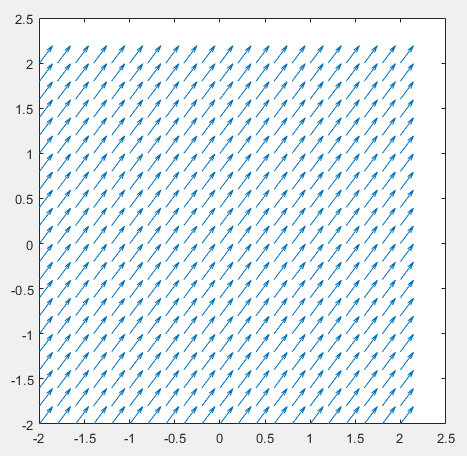
\includegraphics[width = 0.5\textwidth]{example_vector_field_1}
}
\end{tabular}

\begin{tabular}{cc}
\parbox{0.5\textwidth}{
On the right, the vector field
\[\mathbf{F}(x,y) = \begin{bmatrix} 1 \\ x - 1 \end{bmatrix}\]
is depicted. The \(x\) component is constant, so the horizontal component of each arrow is constant. The vertical component increases with \(x\), passing \(0\) when \(x = 1\). The arrows are horizontal when \(x = 1\).
} & \parbox{0.5\textwidth}{
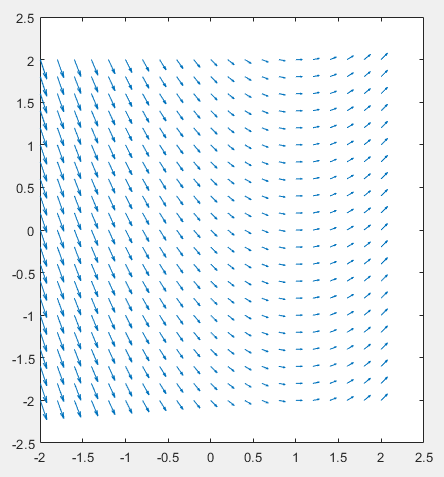
\includegraphics[width = 0.5\textwidth]{example_vector_field_2}
}
\end{tabular}

\begin{tabular}{cc}
\parbox{0.5\textwidth}{
On the right, the vector field
\[\mathbf{F}(x,y) = \begin{bmatrix} x \\ y \end{bmatrix}\]
is depicted. The arrow at each point is a miniature representation of that point's displacement from the origin.  
} & \parbox{0.5\textwidth}{
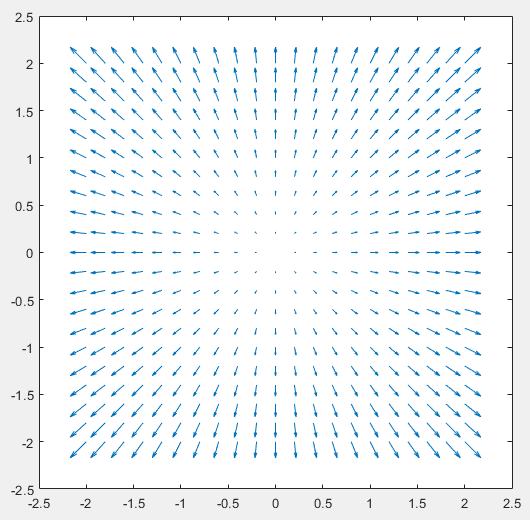
\includegraphics[width = 0.5\textwidth]{example_vector_field_3}
}
\end{tabular}

\begin{tabular}{cc}
\parbox{0.5\textwidth}{
On the right, the vector field
\[\mathbf{F}(x,y) = \begin{bmatrix} y \\ x \end{bmatrix}\]
is depicted. The arrows in quadrants II and IV point towards the origin, while the arrows in quadrants I and III point away from the origin. 
} & \parbox{0.5\textwidth}{
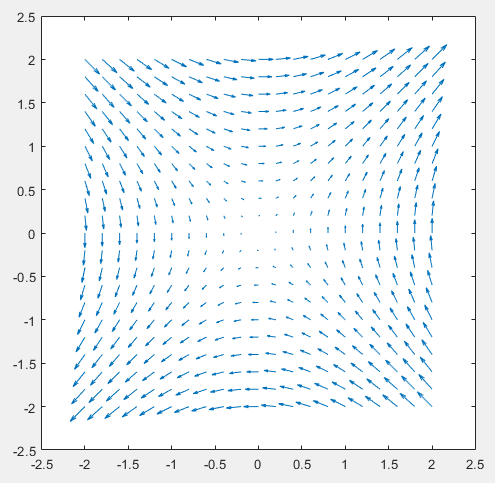
\includegraphics[width = 0.5\textwidth]{example_vector_field_4}
}
\end{tabular}

\begin{tabular}{cc}
\parbox{0.5\textwidth}{
On the right, the vector field
\[\mathbf{F}(x,y) = \begin{bmatrix} -y \\ x \end{bmatrix}\]
is depicted. The arrows point around the origin in a counterclockwise direction, and the length of each arrow is proportional to its distance from the origin.  
} & \parbox{0.5\textwidth}{
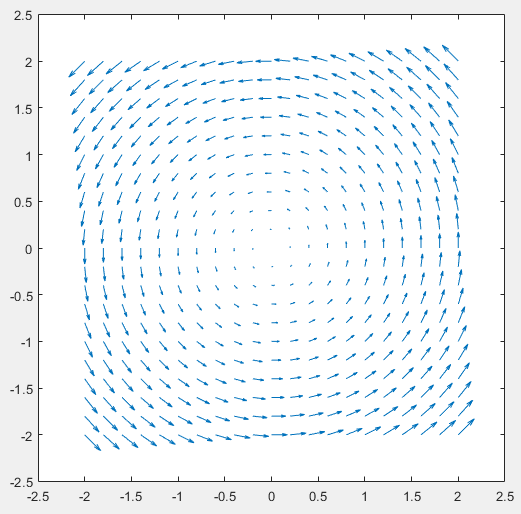
\includegraphics[width = 0.5\textwidth]{example_vector_field_5}
}
\end{tabular}

\begin{tabular}{cc}
\parbox{0.5\textwidth}{
On the right, the vector field 
\[\mathbf{F}(x,y) = \begin{bmatrix} x - y \\ y + x \end{bmatrix}\]
is depicted. This vector field is the sum of the vector fields \(\mathbf{F}_1(x,y) = \begin{bmatrix} x \\ y \end{bmatrix}\) and \(\mathbf{F}_2(x,y) = \begin{bmatrix} -y \\ x \end{bmatrix}\)    
} & \parbox{0.5\textwidth}{
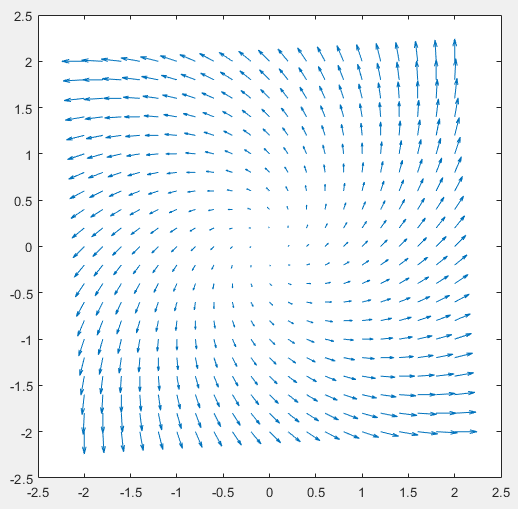
\includegraphics[width = 0.5\textwidth]{example_vector_field_6}
}
\end{tabular}

\begin{tabular}{cc}
\parbox{0.5\textwidth}{
On the right, the vector field 
\[\mathbf{F}(x,y) = \begin{bmatrix} x/\sqrt{x^2 + y^2} \\ y/\sqrt{x^2 + y^2} \end{bmatrix}\]
is depicted. The vectors generated will always have a magnitude of \(1\), and point away from the origin. 
} & \parbox{0.5\textwidth}{
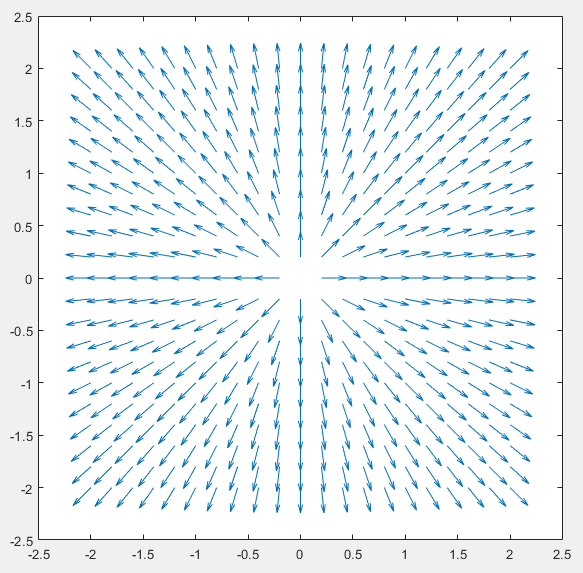
\includegraphics[width = 0.5\textwidth]{example_vector_field_7}
}
\end{tabular}

\begin{tabular}{cc}
\parbox{0.5\textwidth}{
On the right, the vector field 
\[\mathbf{F}(x,y,z) = \begin{bmatrix} -x \\ -y \\ z/\sqrt{x^2 + y^2 + 1} \end{bmatrix}\]
is depicted. This vector field is 3 dimensional. As seen in the image, the vector point towards the \(z\) axis and away from the \(xy\)-plane.
} & \parbox{0.5\textwidth}{
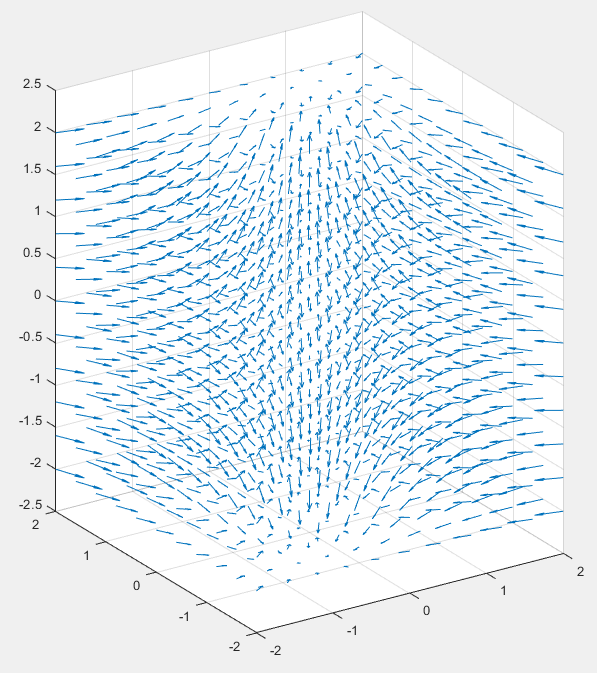
\includegraphics[width = 0.5\textwidth]{example_vector_field_8}
}
\end{tabular}




\section*{Line integrals}

\begin{tabular}{cc}
\parbox{0.5\textwidth}{
A curve \(C\) is {\bf oriented} if and only if it has a preferred direction. In the image on the right, the left hand curve is unoriented, in the sense that there is no preferred direction. The right hand curve is oriented with the preferred direction highlighted with the arrow heads. When curve \(C\) has the parameterization:
\[\mathbf{q}_C(t) \quad\text{where}\quad (a \leq t \leq b)\]
then the ``start" occurs when \(t = a\), and the ``end" occurs when \(t = b\).
} & \parbox{0.5\textwidth}{
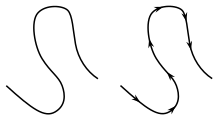
\includegraphics[width = 0.5\textwidth]{unoriented_vs_oriented_curves}
}
\end{tabular}

\begin{tabular}{cc}
\parbox{0.5\textwidth}{
The {\bf line integral} is an integral where the domain of integration is a curve (unoriented or oriented). There are two variants of line integrals. There are scalar line integrals of scalar valued functions \(f(\mathbf{q})\) and vector line integrals of vector valued functions \(\mathbf{F}(\mathbf{q})\). Scalar line integrals {\bf do not} require that the curve be oriented, while vector line integrals require the curve to be oriented. A line integral sees the curve \(C\) partitioned into a large number \(N\) of infinitely small sections. Let the \(i^{\text{th}}\) section contain the representative point \(\mathbf{q}_i^*\). Let the length of the \(i^{\text{th}}\) section be \(\Delta s_i\), which will be important for scalar line integrals. Let the displacement spanned by the \(i^{\text{th}}\) section be \(\Delta \mathbf{q}_i\), which will be important for vector line integrals. An orientation is important to establish the direction of \(\Delta\mathbf{q}_i\). 
} & \parbox{0.5\textwidth}{
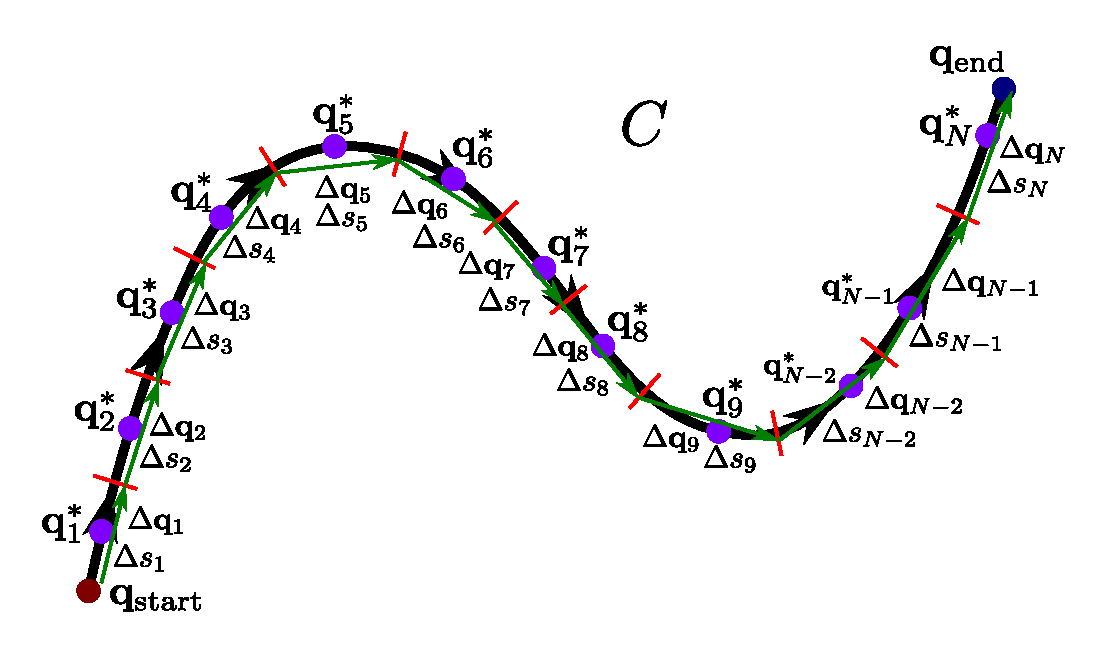
\includegraphics[width = 0.5\textwidth]{line_integral_Riemann_sum}
}
\end{tabular}

The Riemann sum that establishes the scalar line integral of a scalar valued function \(f(\mathbf{q})\) is:
\[\int_C f(\mathbf{q})ds= \lim_{N \rightarrow +\infty} \sum_{i = 1}^N f(\mathbf{q}_i^*) \Delta s_i\]

The Riemann sum that establishes the vector line integral of a vector valued function \(\mathbf{F}(\mathbf{q})\) is:
\[\int_C \mathbf{F}(\mathbf{q}) \bullet d\mathbf{q} = \lim_{N \rightarrow +\infty} \sum_{i = 1}^N \mathbf{F}(\mathbf{q}_i^*) \bullet \Delta \mathbf{q}_i\]

Given a curve \(C\) with the parameterization \(\mathbf{q}_C(t)\) where \(a \leq t \leq b\), how can the scalar and vector line integrals \(\int_C f(\mathbf{q})ds\) and \(\int_C \mathbf{F}(\mathbf{q}) \bullet d\mathbf{q}\) be evaluated? Partition the interval \([a, b]\) into a large number \(N\) of intervals. Let the \(i^{\text{th}}\) interval, denoted by \(I_i\), have the representative value \(t_i^*\). Let the width of the \(i^{\text{th}}\) interval be \(\Delta t_i\). The partitioning of the interval \([a, b]\) gives rise to a partitioning of \(C\). The \(i^{\text{th}}\) section of \(C\), denoted by \(C_i\), has the parameterization \(\mathbf{q}_C(t)\) where \(t\) is confined to the interval \(I_i\). The representative point of \(C_i\) is:
\[\mathbf{q}_i^* = \mathbf{q}_C(t_i^*)\]
The displacement \(\Delta\mathbf{q}_i\) spanned by \(C_i\) is approximately: 
\[\Delta\mathbf{q}_i = \left.\frac{d\mathbf{q}_C}{dt}\right|_{t_i^*}\Delta t_i\] 
The length \(\Delta s_i\) of \(C_i\) is approximately: 
\[\Delta s_i = \left\|\Delta\mathbf{q}_i\right\| = \left\|\left.\frac{d\mathbf{q}_C}{dt}\right|_{t_i^*}\Delta t_i\right\| = \left\|\left.\frac{d\mathbf{q}_C}{dt}\right|_{t_i^*}\right\|\Delta t_i\]       

The scalar line integral \(\int_C f(\mathbf{q})ds\) computed by the Riemann sum is: 
\begin{align*}
\int_C f(\mathbf{q})ds 
= & \lim_{N \rightarrow +\infty} \sum_{i=1}^N f(\mathbf{q}_i^*) \Delta s_i \\ 
= & \lim_{N \rightarrow +\infty} \sum_{i=1}^N f(\mathbf{q}_C(t_i^*)) \left\|\left.\frac{d\mathbf{q}_C}{dt}\right|_{t_i^*}\right\|\Delta t_i \\   
= & \int_{t = a}^b f(\mathbf{q}_C(t)) \left\|\left.\frac{d\mathbf{q}_C}{dt}\right|_{t}\right\| dt  
\end{align*}
Therefore:
\[\int_C f(\mathbf{q})ds = \int_{t = a}^b f(\mathbf{q}_C(t)) \left\|\left.\frac{d\mathbf{q}_C}{dt}\right|_{t}\right\| dt\]

The vector line integral \(\int_C \mathbf{F}(\mathbf{q}) \bullet d\mathbf{q}\) computed by the Riemann sum is: 
\begin{align*}
\int_C \mathbf{F}(\mathbf{q}) \bullet d\mathbf{q} 
= & \lim_{N \rightarrow +\infty} \sum_{i=1}^N \mathbf{F}(\mathbf{q}_i^*) \bullet \Delta \mathbf{q}_i \\ 
= & \lim_{N \rightarrow +\infty} \sum_{i=1}^N \mathbf{F}(\mathbf{q}_C(t_i^*)) \bullet \left.\frac{d\mathbf{q}_C}{dt}\right|_{t_i^*} \Delta t_i \\   
= & \int_{t = a}^b \mathbf{F}(\mathbf{q}_C(t)) \bullet \left.\frac{d\mathbf{q}_C}{dt}\right|_{t} dt  
\end{align*}
Therefore:
\[\int_C \mathbf{F}(\mathbf{q}) \bullet d\mathbf{q} = \int_{t = a}^b \mathbf{F}(\mathbf{q}_C(t)) \bullet \left.\frac{d\mathbf{q}_C}{dt}\right|_{t} dt\]

While the vector line integral of the vector field \(\mathbf{F}(x, y) = \begin{bmatrix} F_x(x, y) \\ F_y(x, y) \end{bmatrix}\) over the oriented curve \(C\) is often denoted via \(\int_C \begin{bmatrix} F_x(x, y) \\ F_y(x, y) \end{bmatrix} \bullet d\mathbf{q}\), the infinitesimal displacement \(d\mathbf{q}\) is equal to \(\begin{bmatrix} dx \\ dy \end{bmatrix}\) where \(dx\) and \(dy\) are the infinitesimal changes in \(x\) and \(y\) respectively. The dot product with \(d\mathbf{q}\) can be expanded to give:
\[\int_C \begin{bmatrix} F_x(x, y) \\ F_y(x, y) \end{bmatrix} \bullet d\mathbf{q} = \int_C \begin{bmatrix} F_x(x, y) \\ F_y(x, y) \end{bmatrix} \bullet \begin{bmatrix} dx \\ dy \end{bmatrix} = \int_C (F_x(x,y)dx + F_y(x,y)dy)\]
The vector line integral in 2 dimensions will often be denoted via the notation \(\int_C (F_x(x,y)dx + F_y(x,y)dy)\). {\bf This is not the sum of two single variable integrals, but a vector line integral.} 

In 3 dimensions, 
\[\int_C \begin{bmatrix} F_x(x, y, z) \\ F_y(x, y, z) \\ F_z(x, y, z) \end{bmatrix} \bullet d\mathbf{q} = \int_C \begin{bmatrix} F_x(x, y, z) \\ F_y(x, y, z) \\ F_z(x, y, z) \end{bmatrix} \bullet \begin{bmatrix} dx \\ dy \\ dz \end{bmatrix} = \int_C (F_x(x,y,z)dx + F_y(x,y,z)dy + F_z(x,y,z)dz)\]

\begin{tabular}{cc}
\parbox{0.5\textwidth}{
A ``piecewise" curve is a curve that consists of multiple component curves linked together end to end. The start of each component curve, except the first component curve, begins where the previous curve ends. Given the \(n\) curves \(C_1, C_2, ..., C_n\), where the curves link together in sequence, the notation \(C_1 + C_2 + ... + C_n\) will denote the piecewise curve constructed from the curves \(C_1, C_2, ..., C_n\). 
Moreover, given the oriented curve \(C\), the notation \(-C\) will denote curve \(C\) with the orientation reversed. 
} & \parbox{0.5\textwidth}{
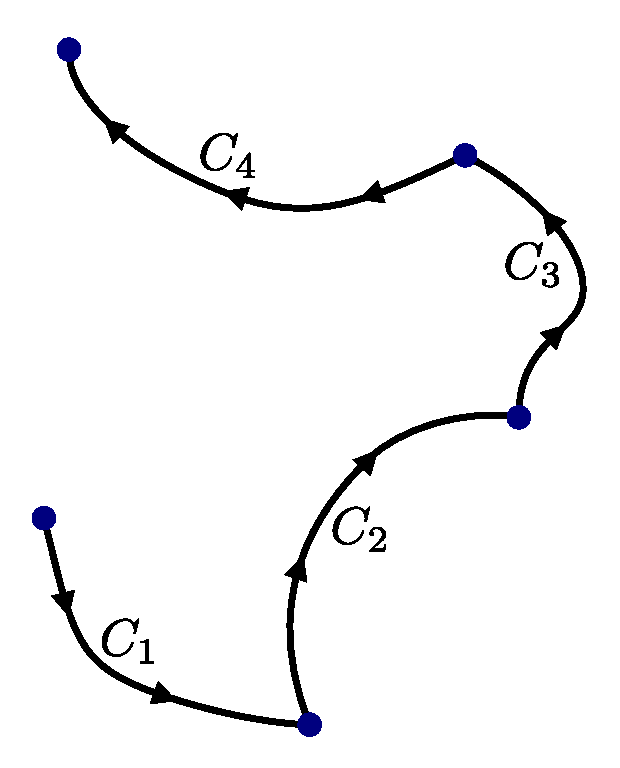
\includegraphics[width = 0.5\textwidth]{piecewise_curve}
}
\end{tabular}

Line integrals along piecewise curves are the sum of the line integrals along their components:
\[\int_{C_1 + C_2 + ... + C_n} f(\mathbf{q})ds = \int_{C_1} f(\mathbf{q})ds + \int_{C_2} f(\mathbf{q})ds + ... + \int_{C_n} f(\mathbf{q})ds\]
\[\int_{C_1 + C_2 + ... + C_n} \mathbf{F}(\mathbf{q}) \bullet d\mathbf{q} = \int_{C_1} \mathbf{F}(\mathbf{q}) \bullet d\mathbf{q} + \int_{C_2} \mathbf{F}(\mathbf{q}) \bullet d\mathbf{q} + ... + \int_{C_n} \mathbf{F}(\mathbf{q}) \bullet d\mathbf{q}\]
Reversing the orientation of curve flips the sign of any vector line integral along said curve:
\[\int_{-C} \mathbf{F}(\mathbf{q}) \bullet d\mathbf{q} = -\int_C \mathbf{F}(\mathbf{q}) \bullet d\mathbf{q}\]


\begin{tabular}{cc}
\parbox{0.5\textwidth}{
The computation of a vector line integral can be visualized by drawing the curve against the quiver plot, as depicted on the right. The curve is oriented from the bottom left to the top right. 

When the curve is moving against the arrows, the dot product of the vector field and displacement differential, \(\mathbf{F}(\mathbf{q}) \bullet d\mathbf{q}\), is negative and subtracts from \(\int_C \mathbf{F}(\mathbf{q}) \bullet d\mathbf{q}\). This is the blue portion of the curve.

When the curve is moving perpendicular to the arrows, the dot product of the vector field and displacement differential, \(\mathbf{F}(\mathbf{q}) \bullet d\mathbf{q}\), is \(0\) and does not affect \(\int_C \mathbf{F}(\mathbf{q}) \bullet d\mathbf{q}\). This is the black portion of the curve. 

When the curve is moving with the arrows, the dot product of the vector field and displacement differential, \(\mathbf{F}(\mathbf{q}) \bullet d\mathbf{q}\), is positive and adds to \(\int_C \mathbf{F}(\mathbf{q}) \bullet d\mathbf{q}\). This is the red portion of the curve. 
} & \parbox{0.5\textwidth}{
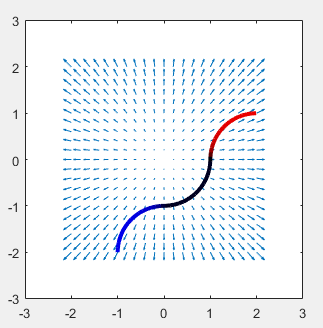
\includegraphics[width = 0.5\textwidth]{example_vector_line_integral_1.png}
}
\end{tabular}

\vspace{5mm}

If \(\mathbf{F}(\mathbf{q})\) denotes force, then the vector line integral \(\int_C \mathbf{F}(\mathbf{q}) \bullet d\mathbf{q}\) is the total energy transferred to any particle that that traverses path \(C\) in the preferred direction. If \(\mathbf{F}(\mathbf{q})\) points against the curve, then the particle is slowed; when \(\mathbf{F}(\mathbf{q})\) points with the curve, then the particle is accelerated; and when \(\mathbf{F}(\mathbf{q})\) is perpendicular to the curve, then the particle is unaffected.


\vspace{5mm}

\textbf{Examples:}**
\begin{itemize}
%%%%%%%%%%%%%%%%%%%%%%%%
\item 
Find the scalar line integral: 
\[\int_C x ds\]
where the curve \(C\) is:
\[C : \quad 
\mathbf{q}_C(t) = \begin{bmatrix} 
t \\ t^2 
\end{bmatrix} \quad 
(0 \leq t \leq 1)\]

The velocity is:
\[\frac{d\mathbf{q}_C}{dt} = \begin{bmatrix} 1 \\ 2t \end{bmatrix}\]
The speed is:
\[\left\|\frac{d\mathbf{q}_C}{dt}\right\| = \sqrt{1 + 4t^2}\]
The integral is:
\begin{align*}
\int_C x ds = & \int_{t = 0}^1 t \cdot (\sqrt{1 + 4t^2} \cdot dt) 
= \int_{t = 0}^1 \frac{1}{8}\sqrt{1 + 4t^2} \cdot (8t dt) 
= \frac{1}{12}(1 + 4t^2)^{3/2} \bigg|_{t=0}^1 \\
= & \frac{1}{12}5^{3/2} - \frac{1}{12} 
= \frac{5^{3/2} - 1}{12}
\end{align*}

%%%%%%%%%%%%%%%%%%%%%%%%
\item** 
Find the scalar line integral: 
\[\int_C xy^4 ds\]
where the curve \(C\) is:
\[C : \quad 
\mathbf{q}_C(t) = \begin{bmatrix} 
2\sin(t) \\ 2\cos(t) 
\end{bmatrix} \quad 
(0 \leq t \leq \pi)\]

The velocity is:
\[\frac{d\mathbf{q}_C}{dt} = \begin{bmatrix} 2\cos(t) \\ -2\sin(t) \end{bmatrix}\]
The speed is:
\[\left\|\frac{d\mathbf{q}_C}{dt}\right\| = \sqrt{4\cos^2(t) + 4\sin^2(t)} = \sqrt{4} = 2\]
The integral is:
\begin{align*}
\int_C xy^4 ds 
= & \int_{t = 0}^{\pi} (2\sin(t))(2\cos(t))^4 \cdot (2dt) 
= \int_{t = 0}^{\pi} 64 \sin(t) \cos^4(t) dt  
= \int_{t = 0}^{\pi} -64 \cos^4(t) (-\sin(t) dt) \\ 
= & -\frac{64}{5}\cos^5(t) \bigg|_{t = 0}^{\pi} 
= (-\frac{64}{5}(-1)^5) - (-\frac{64}{5}1^5) 
= \frac{64}{5} + \frac{64}{5} 
= \frac{128}{5}
\end{align*}

%%%%%%%%%%%%%%%%%%%%%%%%
\item
Find the scalar line integral: 
\[\int_C (4x + 3y)ds\]
where the curve \(C\) is:
\[C : \quad 
\mathbf{q}_C(t) = \begin{bmatrix} 
2 - t \\ -1 + 2t \\ 3 - 2t
\end{bmatrix} \quad 
(0 \leq t \leq 1)\]

The velocity is:
\[\frac{d\mathbf{q}_C}{dt} = \begin{bmatrix} -1 \\ 2 \\ -2 \end{bmatrix}\]
The speed is:
\[\left\|\frac{d\mathbf{q}_C}{dt}\right\| 
= \sqrt{1 + 4 + 4}
= \sqrt{9} = 3\]
The integral is:
\begin{align*}
\int_C (4x + 3y)ds = & \int_{t = 0}^1 (4(2 - t) + 3(-1 + 2t)) \cdot (3dt) 
= \int_{t = 0}^1 3((8 - 4t) + (-3 + 6t)) dt 
= \int_{t = 0}^1 3(5 + 2t) dt \\
= & \int_{t = 0}^1 (15 + 6t) dt 
= (15t + 3t^2)\Big|_{t=0}^1 
= 18
\end{align*}

%%%%%%%%%%%%%%%%%%%%%%%%
\item**
Find the scalar line integral: 
\[\int_C \frac{ds}{x^2 + y^2 + z^2}\]
where the curve \(C\) is:
\[C : \quad 
\mathbf{q}_C(t) = \begin{bmatrix} 
\cos(t) \\ \sin(t) \\ t
\end{bmatrix} \quad 
(0 \leq t \leq 1)\]

The velocity is:
\[\frac{d\mathbf{q}_C}{dt} = \begin{bmatrix} 
-\sin(t) \\ \cos(t) \\ 1
\end{bmatrix}\]
The speed is:
\[\left\|\frac{d\mathbf{q}_C}{dt}\right\| = \sqrt{\sin^2(t) + \cos^2(t) + 1} = \sqrt{1 + 1} = \sqrt{2}\]
The integral is:
\begin{align*}
\int_C \frac{ds}{x^2 + y^2 + z^2} 
= & \int_{t = 0}^1 \frac{1}{\cos^2(t) + \sin^2(t) + t^2} \cdot (\sqrt{2} dt) 
= \int_{t = 0}^1 \frac{\sqrt{2}}{t^2 + 1} dt \\ 
= & \sqrt{2} \cdot \tan^{-1}(t)\Big|_{t = 0}^1 
= \sqrt{2} \cdot \frac{\pi}{4} - 0 
= \frac{\pi}{2\sqrt{2}}
\end{align*}

%%%%%%%%%%%%%%%%%%%%%%%%
\item
Find the scalar line integral: 
\[\int_C (x + y) ds\]
where the curve \(C\) is:
\[C : \quad 
\mathbf{q}_C(t) = \begin{bmatrix} 
3\cos(2t) \\ 4 \\ -3\sin(2t) 
\end{bmatrix} \quad 
(0 \leq t \leq \frac{\pi}{2})\]

The velocity is:
\[\frac{d\mathbf{q}_C}{dt} = \begin{bmatrix} -6\sin(2t) \\ 0 \\ -6\cos(2t) \end{bmatrix}\]
The speed is:
\[\left\|\frac{d\mathbf{q}_C}{dt}\right\| 
= \sqrt{36\sin^2(2t) + 0 + 36\cos^2(2t)} 
= \sqrt{36} = 6\] 
The integral is:
\begin{align*}
\int_C (x + y) ds = & \int_{t = 0}^{\pi/2} (3\cos(2t) + 4) \cdot (6dt) 
= \int_{t = 0}^{\pi/2} (18\cos(2t) + 24) dt \\  
= & (9\sin(2t) + 24t)\bigg|_{t = 0}^{\pi/2} 
= (9\sin(\pi) + 12\pi) - (0 + 0) 
= 12\pi
\end{align*}

%%%%%%%%%%%%%%%%%%%%%%%%
\item
Find the scalar line integral: 
\[\int_C x^2 ds\]
where the curve \(C\) is:
\[C : \quad 
\mathbf{q}_C(t) = \begin{bmatrix} 
4\cos(t) \\ 3t \\ 4\sin(t)
\end{bmatrix} \quad 
(0 \leq t \leq 2\pi)\]

The velocity is:
\[\frac{d\mathbf{q}_C}{dt} = \begin{bmatrix} -4\sin(t) \\ 3 \\ 4\cos(t) \end{bmatrix}\]
The speed is:
\[\left\|\frac{d\mathbf{q}_C}{dt}\right\| 
= \sqrt{16\sin^2(t) + 9 + 16\cos^2(t)}
= \sqrt{16 + 9} = \sqrt{25} = 5\]
The integral is:
\begin{align*}
\int_C x^2 ds = & \int_{t = 0}^{2\pi} (4\cos(t))^2 \cdot (5dt) 
= \int_{t = 0}^{2\pi} 80\cos^2(t) dt 
= \int_{t = 0}^{2\pi} 80\frac{1 + \cos(2t)}{2} dt   
= \int_{t = 0}^{2\pi} (40 + 40\cos(2t))dt \\ 
= & (40t + 20\sin(2t))\Big|_{t=0}^{2\pi} 
= (80\pi + 20\sin(4\pi)) - (0 + 20\sin(0)) 
= 80\pi
\end{align*}

%%%%%%%%%%%%%%%%%%%%%%%%
\item**
Find the vector line integral: 
\[\int_C \begin{bmatrix} y^2 \\ x \end{bmatrix} \bullet d\mathbf{q}\]
where the curve \(C\) is:
\[C : \quad 
\mathbf{q}_C(t) = \begin{bmatrix} 
4 - t^2 \\ t 
\end{bmatrix} \quad 
(-3 \leq t \leq 2)\]

The velocity is:
\[\frac{d\mathbf{q}_C}{dt} = \begin{bmatrix} -2t \\ 1 \end{bmatrix}\] 
The integral is:
\begin{align*}
\int_C \begin{bmatrix} y^2 \\ x \end{bmatrix} \bullet d\mathbf{q} = & \int_{t = -3}^2 \begin{bmatrix} t^2 \\ 4 - t^2 \end{bmatrix} \bullet \begin{bmatrix} -2t \\ 1 \end{bmatrix} dt 
= \int_{t = -3}^2 (-2t^3 + (4 - t^2))dt 
= \int_{t = -3}^2 (-2t^3 - t^2 + 4)dt \\   
= & (-\frac{1}{2}t^4 - \frac{1}{3}t^3 + 4t)\Big|_{t = -3}^2 
= (-8 - \frac{8}{3} + 8) - (-\frac{81}{2} + 9 - 12) 
= 3 - \frac{8}{3} + \frac{81}{2} \\ 
= & \frac{18 - 16 + 243}{6} 
= \frac{245}{6}
\end{align*}

%%%%%%%%%%%%%%%%%%%%%%%%
\item
Find the vector line integral: 
\[\int_C \begin{bmatrix} x^2 + y \\ x^2 - y \end{bmatrix} \bullet d\mathbf{q}\]
where the curve \(C\) is:
\[C : \quad 
\mathbf{q}_C(t) = \begin{bmatrix} 
t \\ t^2  
\end{bmatrix} \quad 
(0 \leq t \leq 1)\]

The velocity is:
\[\frac{d\mathbf{q}_C}{dt} = \begin{bmatrix} 1 \\ 2t \end{bmatrix}\]
The integral is:
\begin{align*}
\int_C \begin{bmatrix} x^2 + y \\ x^2 - y \end{bmatrix} \bullet d\mathbf{q} 
= & \int_{t=0}^1 \begin{bmatrix} t^2 + t^2 \\ t^2 - t^2 \end{bmatrix} \bullet \begin{bmatrix} 1 \\ 2t \end{bmatrix} dt   
= \int_{t=0}^1 \begin{bmatrix} 2t^2 \\ 0 \end{bmatrix} \bullet \begin{bmatrix} 1 \\ 2t \end{bmatrix} dt   
= \int_{t=0}^1 2t^2 dt   
= \frac{2}{3}t^3\bigg|_{t=0}^1 
= \frac{2}{3}
\end{align*}

%%%%%%%%%%%%%%%%%%%%%%%%
\item** 
Find the vector line integral: 
\[\int_C \begin{bmatrix} zy \\ x \\ z^2x \end{bmatrix} \bullet d\mathbf{q}\]
where the curve \(C\) is:
\[C : \quad 
\mathbf{q}_C(t) = \begin{bmatrix} 
t \\ 2t \\ 3t  
\end{bmatrix} \quad 
(0 \leq t \leq 1)\]

The velocity is:
\[\frac{d\mathbf{q}_C}{dt} = \begin{bmatrix} 
1 \\ 2 \\ 3  
\end{bmatrix}\]
The integral is:
\begin{align*}
\int_C \begin{bmatrix} zy \\ x \\ z^2x \end{bmatrix} \bullet d\mathbf{q}
= & \int_{t=0}^1 \begin{bmatrix} (3t)(2t) \\ t \\ (3t)^2t \end{bmatrix} \bullet \begin{bmatrix} 1 \\ 2 \\ 3 \end{bmatrix}dt
= \int_{t=0}^1 \begin{bmatrix} 6t^2 \\ t \\ 9t^3 \end{bmatrix} \bullet \begin{bmatrix} 1 \\ 2 \\ 3 \end{bmatrix}dt 
= \int_{t=0}^1 (6t^2 + 2t + 27t^3)dt \\
= & (2t^3 + t^2 + \frac{27}{4}t^4)\bigg|_{t=0}^1 
= (2 + 1 + \frac{27}{4}) - 0 
= \frac{39}{4}
\end{align*}

%%%%%%%%%%%%%%%%%%%%%%%%
\item 
Find the vector line integral: 
\[\int_C \begin{bmatrix} -(5y + 4)/2 \\ \sqrt{2x} - 3 \end{bmatrix} \bullet d\mathbf{q}\]
where the curve \(C\) is:
\[C : \quad 
\mathbf{q}_C(t) = \begin{bmatrix} 
(1/2)t^2 \\ -2t   
\end{bmatrix} \quad 
(0 \leq t \leq 3)\]

The velocity is:
\[\frac{d\mathbf{q}_C}{dt} = \begin{bmatrix} t \\ -2 \end{bmatrix}\]
The integral is:
\begin{align*}
\int_C \begin{bmatrix} -(5y + 4)/2 \\ \sqrt{2x} - 3 \end{bmatrix} \bullet d\mathbf{q} 
= & \int_{t = 0}^3 \begin{bmatrix} -(5(-2t) + 4)/2 \\ \sqrt{2((1/2)t^2)} - 3 \end{bmatrix} \bullet \begin{bmatrix} t \\ -2 \end{bmatrix} dt  
= \int_{t = 0}^3 \begin{bmatrix} (10t - 4)/2 \\ \sqrt{t^2} - 3 \end{bmatrix} \bullet \begin{bmatrix} t \\ -2 \end{bmatrix} dt \\ 
= & \int_{t = 0}^3 \begin{bmatrix} 5t - 2 \\ t - 3 \end{bmatrix} \bullet \begin{bmatrix} t \\ -2 \end{bmatrix} dt  
= \int_{t = 0}^3 ((5t^2 - 2t) + (-2t + 6))dt  
= \int_{t = 0}^3 (5t^2 - 4t + 6)dt \\ 
= & (\frac{5}{3}t^3 - 2t^2 + 6t)\Big|_{t=0}^3 
= (45 - 18 + 18) - 0 = 45
\end{align*}

%%%%%%%%%%%%%%%%%%%%%%%%
\item 
Find the vector line integral: 
\[\int_C \begin{bmatrix} y \\ -2x \\ z \end{bmatrix} \bullet d\mathbf{q}\]
where the curve \(C\) is:
\[C : \quad 
\mathbf{q}_C(t) = \begin{bmatrix} 
-1 + \sin(t) \\ -1 - \cos(t) \\ 2t  
\end{bmatrix} \quad 
(0 \leq t \leq \pi)\]

The velocity is:
\[\frac{d\mathbf{q}_C}{dt} = \begin{bmatrix} 
\cos(t) \\ \sin(t) \\ 2  
\end{bmatrix}\]
The integral is:
\begin{align*}
\int_C \begin{bmatrix} y \\ -2x \\ z \end{bmatrix} \bullet d\mathbf{q} 
= & \int_{t=0}^{\pi} \begin{bmatrix} -1 - \cos(t) \\ -2(-1 + \sin(t)) \\ 2t \end{bmatrix} \bullet \begin{bmatrix} 
\cos(t) \\ \sin(t) \\ 2  
\end{bmatrix}dt
= \int_{t=0}^{\pi} \begin{bmatrix} -1 - \cos(t) \\ 2 - 2\sin(t) \\ 2t \end{bmatrix} \bullet \begin{bmatrix} 
\cos(t) \\ \sin(t) \\ 2  
\end{bmatrix}dt \\ 
= & \int_{t=0}^{\pi} ((-\cos^2(t) - \cos(t)) + (-2\sin^2(t) + 2\sin(t)) + 4t)dt \\ 
= & \int_{t=0}^{\pi} ((-\frac{1 + \cos(2t)}{2} - \cos(t)) + (-2\frac{1 - \cos(2t)}{2} + 2\sin(t)) + 4t)dt \\ 
= & \int_{t=0}^{\pi} ((-\frac{1}{2} - \cos(t) - \frac{1}{2}\cos(2t)) + (-1 + 2\sin(t) + \cos(2t)) + 4t)dt \\ 
= & \int_{t=0}^{\pi} (-\frac{3}{2} - \cos(t) + 2\sin(t) + \frac{1}{2}\cos(2t) + 4t)dt \\ 
= & (-\frac{3}{2}t - \sin(t) - 2\cos(t) + \frac{1}{4}\sin(2t) + 2t^2)\bigg|_{t=0}^{\pi} \\
= & (-\frac{3}{2}\pi - 0 - 2(-1) + \frac{1}{4}(0) + 2\pi^2) - (-\frac{3}{2}(0) - 0 - 2(1) + \frac{1}{4}(0) + 2(0)^2) \\
= & (2 - \frac{3}{2}\pi + 2\pi^2) - (-2) 
= 4 - \frac{3}{2}\pi + 2\pi^2
\end{align*}

%%%%%%%%%%%%%%%%%%%%%%%%
\item 
Find the vector line integral: 
\[\int_C \begin{bmatrix} -y \\ x \\ 1/(z + 1) \end{bmatrix} \bullet d\mathbf{q}\]
where the curve \(C\) is:
\[C : \quad 
\mathbf{q}_C(t) = \begin{bmatrix} 
2 - t \\ 3t - (3/4)t^2 \\ (3/2)t  
\end{bmatrix} \quad 
(0 \leq t \leq 2)\] 

The velocity is:
\[\frac{d\mathbf{q}_C}{dt} = \begin{bmatrix} 
-1 \\ 3 - (3/2)t \\ 3/2  
\end{bmatrix}\]
The integral is:
\begin{align*}
\int_C \begin{bmatrix} -y \\ x \\ 1/(z + 1) \end{bmatrix} \bullet d\mathbf{q} 
= & \int_{t=0}^2 \begin{bmatrix} -(3t - (3/4)t^2) \\ 2 - t \\ 1/((3/2)t + 1) \end{bmatrix} \bullet \begin{bmatrix} 
-1 \\ 3 - (3/2)t \\ 3/2  
\end{bmatrix}dt \\ 
= & \int_{t=0}^2 ((3t - (3/4)t^2) + ((3/2)t^2 - 6t + 6) + \frac{3}{3t + 2})dt \\ 
= & \int_{t=0}^2 ((3/4)t^2 - 3t + 6 + \frac{3}{3t + 2})dt   
= (\frac{1}{4}t^3 - \frac{3}{2}t^2 + 6t + \ln|3t + 2|)\bigg|_{t=0}^2 \\ 
= & (2 - 6 + 12 + \ln(8)) - (0 - 0 + 0 + \ln(2)) 
= 8 + \ln(4)
\end{align*}

\end{itemize}
**Examples are from: \\
Strang, G. et. al., ``Calculus Volume 3", \emph{Openstax}, Chapter 6.2 





\section*{The gradient theorem}

Given a single differentiable single variable function \(g(x)\) over the interval \([a, b]\), the fundamental theorem of calculus gives:
\[\int_{x = a}^b \frac{dg}{dx}dx = g(b) - g(a)\]
A similar theorem holds for multivariable functions. 

Given a scalar valued multivariable function \(f(\mathbf{q})\), the gradient \(\nabla f = \begin{bmatrix} \partial f/\partial x \\ \partial f/\partial y \\ \partial f/\partial z \end{bmatrix}\) is itself a vector field. Let \(C\) denote an oriented curve with a starting point of \(\mathbf{q}_{\text{start}}\) and an ending point of \(\mathbf{q}_{\text{end}}\). Let \(C\) have the parameterization \(\mathbf{q}_C(t) = \begin{bmatrix} x_C(t) \\ y_C(t) \\ z_C(t) \end{bmatrix}\) where \(a \leq t \leq b\). It is clear that \(\mathbf{q}_{\text{start}} = \mathbf{q}_C(a)\) and \(\mathbf{q}_{\text{end}} = \mathbf{q}_C(b)\). 

Define the single variable function \(g(t)\) with the domain \([a, b]\) via:
\[g(t) = f(\mathbf{q}_C(t)) = f(x_C(t), y_C(t), z_C(t))\]
The multivariable chain rule gives: 
\begin{align*}
\frac{dg}{dt} 
= & \frac{\partial f}{\partial x}\bigg|_{\mathbf{q}_C(t)}\frac{dx_C}{dt} + \frac{\partial f}{\partial y}\bigg|_{\mathbf{q}_C(t)}\frac{dy_C}{dt} + \frac{\partial f}{\partial z}\bigg|_{\mathbf{q}_C(t)}\frac{dz_C}{dt}
= \begin{bmatrix} (\partial f/\partial x)|_{\mathbf{q}_C(t)} \\ (\partial f/\partial y)|_{\mathbf{q}_C(t)} \\ (\partial f/\partial z)|_{\mathbf{q}_C(t)} \end{bmatrix} \bullet \begin{bmatrix} dx_C/dt \\ dy_C/dt \\ dz_C/dt \end{bmatrix} \\
= & (\nabla f)\bigg|_{\mathbf{q}_C(t)} \bullet \frac{d\mathbf{q}_C}{dt}
\end{align*}
The fundamental theorem of calculus gives: 
\begin{align*}
& \int_{t = a}^b \frac{dg}{dt}dt = g(b) - g(a) \\
\iff & \int_{t = a}^b \left((\nabla f)\bigg|_{\mathbf{q}_C(t)} \bullet \frac{d\mathbf{q}_C}{dt}\right)dt = f(\mathbf{q}_C(b)) - f(\mathbf{q}_C(a)) \\ 
\iff & \int_C (\nabla f) \bullet d\mathbf{q} = f(\mathbf{q}_{\text{end}}) - f(\mathbf{q}_{\text{start}})
\end{align*}
The equation: 
\[\int_C (\nabla f) \bullet d\mathbf{q} = f(\mathbf{q}_{\text{end}}) - f(\mathbf{q}_{\text{start}})\]
is the multivariable analog to the fundamental theorem of calculus, and is often referred to as the {\bf gradient theorem}, or the {\bf fundamental theorem of line integrals}. 

Consider trying to compute the vector line integral \(\int_C \mathbf{F}(\mathbf{q}) \bullet d\mathbf{q}\). If a multivariable scalar valued function \(f(\mathbf{q})\), referred to a {\bf potential function}, can be found such that \(\nabla f = \mathbf{F}\), then computing vector line integrals is easy using the gradient theorem:
\[\int_C \mathbf{F}(\mathbf{q}) \bullet d\mathbf{q} = f(\mathbf{q}_{\text{end}}) - f(\mathbf{q}_{\text{start}})\]
All that is needed are the endpoints of \(C\). The intermediate points of \(C\) don't matter. 

A potential function \(f(\mathbf{q})\) where \(\nabla f = \mathbf{F}(\mathbf{q})\) does not always exist. For example, the vector field \(\mathbf{F}(x,y) = \begin{bmatrix} -y \\ x \end{bmatrix}\) does not have a potential function. If the potential function exists, then the vector field \(\mathbf{F}(\mathbf{q})\) is said to be {\bf conservative}. Since the vector line integrals of conservative vector fields depend only on the endpoints of the oriented curve being integrated over, conservative vector fields are also referred to as being {\bf path independent}. The vector line integrals of conservative vector fields around closed loops is \(0\), so conservative vector fields are also referred to as being {\bf irrotational}. 

How can one determine if a vector field is conservative? If \(\mathbf{F}(x,y,z) = \begin{bmatrix} F_x(x,y,z) \\ F_y(x,y,z) \\ F_z(x,y,z) \end{bmatrix}\) is the gradient of a scalar valued function \(f(x,y,z)\), then the following properties must hold. 

By definition \(F_x(x,y,z) = \frac{\partial f}{\partial x}\); \(F_y(x,y,z) = \frac{\partial f}{\partial y}\); and \(F_z(x,y,z) = \frac{\partial f}{\partial z}\). 

Since mixed second order partial derivatives do not depend of the order in which the derivatives are applied:
\[\frac{\partial^2 f}{\partial y \partial x} = \frac{\partial^2 f}{\partial x \partial y} \quad\implies\quad \frac{\partial}{\partial y}\left(\frac{\partial f}{\partial x}\right) = \frac{\partial}{\partial x}\left(\frac{\partial f}{\partial y}\right) \quad\implies\quad \frac{\partial F_x}{\partial y} = \frac{\partial F_y}{\partial x}\]
\[\frac{\partial^2 f}{\partial z \partial x} = \frac{\partial^2 f}{\partial x \partial z} \quad\implies\quad \frac{\partial}{\partial z}\left(\frac{\partial f}{\partial x}\right) = \frac{\partial}{\partial x}\left(\frac{\partial f}{\partial z}\right) \quad\implies\quad \frac{\partial F_x}{\partial z} = \frac{\partial F_z}{\partial x}\]
\[\frac{\partial^2 f}{\partial z \partial y} = \frac{\partial^2 f}{\partial y \partial z} \quad\implies\quad \frac{\partial}{\partial z}\left(\frac{\partial f}{\partial y}\right) = \frac{\partial}{\partial y}\left(\frac{\partial f}{\partial z}\right) \quad\implies\quad \frac{\partial F_y}{\partial z} = \frac{\partial F_z}{\partial y}\]
{\bf In conclusion, a vector field \(\mathbf{F}(x,y,z) = \begin{bmatrix} F_x(x,y,z) \\ F_y(x,y,z) \\ F_z(x,y,z) \end{bmatrix}\) is conservative if and only if} 
\[\frac{\partial F_x}{\partial y} = \frac{\partial F_y}{\partial x} 
\quad\text{and}\quad 
\frac{\partial F_x}{\partial z} = \frac{\partial F_z}{\partial x} 
\quad\text{and}\quad 
\frac{\partial F_y}{\partial z} = \frac{\partial F_z}{\partial y}\]
In the case of a 2D vector field, the vector field \(\mathbf{F}(x,y) = \begin{bmatrix} F_x(x,y) \\ F_y(x,y) \end{bmatrix}\) is conservative if and only if 
\[\frac{\partial F_x}{\partial y} = \frac{\partial F_y}{\partial x}\]

\vspace{5mm}

\textbf{Examples:} 
\begin{itemize}
%%%%%%%%%%%%%%%%%%%%
\item Consider the 2D vector field \(\mathbf{F}(x,y) = \begin{bmatrix} -y \\ x \end{bmatrix}\). The components are \(F_x(x,y) = -y\) and \(F_y(x,y) = x\), so \(\frac{\partial F_x}{\partial y} = -1\) and \(\frac{\partial F_y}{\partial x} = 1\). 

\(\frac{\partial F_x}{\partial y} \neq \frac{\partial F_y}{\partial x}\) so this vector field is not conservative.  
%%%%%%%%%%%%%%%%%%%%
\item Consider the 3D vector field \(\mathbf{F}(x,y,z) = \begin{bmatrix} yz \\ xz \\ xy \end{bmatrix}\). The components are \(F_x(x,y,z) = yz\) and \(F_y(x,y,z) = xz\) and \(F_z(x,y,z) = xy\). 

Checking if the vector field is conservative:
\[\frac{\partial F_x}{\partial y} = z \quad\quad\text{and}\quad\quad \frac{\partial F_y}{\partial x} = z \quad\quad\text{so}\quad\quad \frac{\partial F_x}{\partial y} = \frac{\partial F_y}{\partial x}\]
\[\frac{\partial F_x}{\partial z} = y \quad\quad\text{and}\quad\quad \frac{\partial F_z}{\partial x} = y \quad\quad\text{so}\quad\quad \frac{\partial F_x}{\partial z} = \frac{\partial F_z}{\partial x}\]
\[\frac{\partial F_y}{\partial z} = x \quad\quad\text{and}\quad\quad \frac{\partial F_z}{\partial y} = x \quad\quad\text{so}\quad\quad \frac{\partial F_y}{\partial z} = \frac{\partial F_z}{\partial y}\]

All tests pass, so the vector field is conservative.
%%%%%%%%%%%%%%%%%%%%
\item Consider the 3D vector field \(\mathbf{F}(x,y,z) = \begin{bmatrix} -3y \\ -3x \\ -3y \end{bmatrix}\). The components are \(F_x(x,y,z) = -3y\) and \(F_y(x,y,z) = -3x\) and \(F_z(x,y,z) = -3z\). 

Checking if the vector field is conservative:
\[\frac{\partial F_x}{\partial y} = -3 \quad\quad\text{and}\quad\quad \frac{\partial F_y}{\partial x} = -3 \quad\quad\text{so}\quad\quad \frac{\partial F_x}{\partial y} = \frac{\partial F_y}{\partial x}\]
\[\frac{\partial F_x}{\partial z} = 0 \quad\quad\text{and}\quad\quad \frac{\partial F_z}{\partial x} = 0 \quad\quad\text{so}\quad\quad \frac{\partial F_x}{\partial z} = \frac{\partial F_z}{\partial x}\]
\[\frac{\partial F_y}{\partial z} = 0 \quad\quad\text{and}\quad\quad \frac{\partial F_z}{\partial y} = -3 \quad\quad\text{so}\quad\quad \frac{\partial F_y}{\partial z} \neq \frac{\partial F_z}{\partial y}\]

The \(3^{\text{rd}}\) test fails, so the vector field is not conservative.
\end{itemize}

\vspace{5mm}

\begin{tabular}{cc}
\parbox{0.5\textwidth}{
Once a vector field \(\mathbf{F}(x,y,z) = \begin{bmatrix} F_x(x,y,z) \\ F_y(x,y,z) \\ F_z(x,y,z) \end{bmatrix}\) has been confirmed to be conservative, the task is now to find a potential function \(f(x,y,z)\). To find a scalar potential function, the gradient theorem will be used. Let \((x,y,z)\) be an arbitrary point. Consider the piecewise curve \(C\) depicted on the right. \(C\) consists of 3 components. \(C_x\) is parallel to the \(x\) axis and starts at \((0, 0, 0)\) and ends at \((x, 0, 0)\). \(C_y\) is parallel to the \(y\) axis and starts at \((x, 0, 0)\) and ends at \((x, y, 0)\). \(C_z\) is parallel to the \(z\) axis and starts at \((x, y, 0)\) and ends at \((x, y, z)\). These 3 components have the parameterizations: 
} & \parbox{0.5\textwidth}{
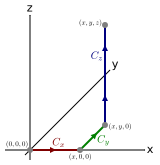
\includegraphics[width = 0.5\textwidth]{finding_the_scalar_potential}
}
\end{tabular}

\[C_x: \quad \mathbf{q}_{x}(t) = \begin{bmatrix} t \\ 0 \\ 0 \end{bmatrix} \quad (0 \leq t \leq x) 
\quad \quad\quad\text{and}\quad\quad\quad   
C_y: \quad \mathbf{q}_{y}(t) = \begin{bmatrix} x \\ t \\ 0 \end{bmatrix} \quad (0 \leq t \leq y)\]
\[\quad\quad\text{and}\quad\quad\quad   
C_z: \quad \mathbf{q}_{z}(t) = \begin{bmatrix} x \\ y \\ t \end{bmatrix} \quad (0 \leq t \leq z)\]

The vector line integral of \(\mathbf{F}(x,y,z) = \begin{bmatrix} F_x(x,y,z) \\ F_y(x,y,z) \\ F_z(x,y,z) \end{bmatrix}\) along \(C = C_x + C_y + C_z\) is: 
\begin{align*}
& \int_{C_x + C_y + C_z} \mathbf{F}(\mathbf{q}) \bullet d\mathbf{q} 
= \int_{C_x} \mathbf{F}(\mathbf{q}) \bullet d\mathbf{q} + \int_{C_y} \mathbf{F}(\mathbf{q}) \bullet d\mathbf{q} + \int_{C_z} \mathbf{F}(\mathbf{q}) \bullet d\mathbf{q} \\
& = \int_{t = 0}^x \mathbf{F}(\mathbf{q}_{x}(t)) \bullet \frac{d\mathbf{q}_x}{dt}dt + \int_{t = 0}^y \mathbf{F}(\mathbf{q}_{y}(t)) \bullet \frac{d\mathbf{q}_y}{dt}dt + \int_{t = 0}^z \mathbf{F}(\mathbf{q}_{z}(t)) \bullet \frac{d\mathbf{q}_z}{dt}dt \\
& = \int_{t = 0}^x \begin{bmatrix} F_x(t,0,0) \\ F_y(t,0,0) \\ F_z(t,0,0) \end{bmatrix} \bullet \begin{bmatrix} 1 \\ 0 \\ 0 \end{bmatrix}dt + \int_{t = 0}^y \begin{bmatrix} F_x(x,t,0) \\ F_y(x,t,0) \\ F_z(x,t,0) \end{bmatrix} \bullet \begin{bmatrix} 0 \\ 1 \\ 0 \end{bmatrix}dt + \int_{t = 0}^z \begin{bmatrix} F_x(x,y,t) \\ F_y(x,y,t) \\ F_z(x,y,t) \end{bmatrix} \bullet \begin{bmatrix} 0 \\ 0 \\ 1 \end{bmatrix}dt \\ 
& = \int_{t = 0}^x F_x(t,0,0)dt + \int_{t = 0}^y F_y(x,t,0)dt + \int_{t = 0}^z F_z(x,y,t)dt
\end{align*}
Choose an arbitrary value \(f_0\) for \(f(0,0,0)\). The gradient theorem yields:
\[\int_{C_x + C_y + C_z} \mathbf{F}(\mathbf{q}) \bullet d\mathbf{q} = f(x,y,z) - f(0,0,0)\]
so therefore the {\bf potential function of the vector field \(\mathbf{F}(x,y,z) = \begin{bmatrix} F_x(x,y,z) \\ F_y(x,y,z) \\ F_z(x,y,z) \end{bmatrix}\) is:}
\[f(x,y,z) = f_0 + \int_{t = 0}^x F_x(t,0,0)dt + \int_{t = 0}^y F_y(x,t,0)dt + \int_{t = 0}^z F_z(x,y,t)dt\]
where \(f_0\) is an arbitrary constant. 


\vspace{5mm}

\textbf{Examples:}

\begin{itemize}
%%%%%%%%%%%%%%%%%%%%%%%%
\item
Find the vector line integral: 
\[\int_C \begin{bmatrix}
3yz \\ 
3xz - 2z \\ 
3xy - 2y
\end{bmatrix} \bullet d\mathbf{q}\]
where the curve \(C\) is:
\[C : \quad \mathbf{q}_C(t) = \begin{bmatrix}
2 - t^2 \\ 
3t - 6 \\ 
t^3 - 2t
\end{bmatrix} \quad 
(1 \leq t \leq 2)\]
 
The vector field is:
\[\mathbf{F}(x,y,z) = \begin{bmatrix}
3yz \\ 
3xz - 2z \\ 
3xy - 2y
\end{bmatrix} \quad\quad\text{and}\quad\quad \begin{array}{l} 
F_x(x,y,z) = 3yz \\ 
F_y(x,y,z) = 3xz - 2z \\ 
F_z(x,y,z) = 3xy - 2y
\end{array}\]

Checking if the vector field is conservative:
\[\frac{\partial F_x}{\partial y} = 3z \quad\quad\text{and}\quad\quad \frac{\partial F_y}{\partial x} = 3z \quad\quad\text{so}\quad\quad \frac{\partial F_x}{\partial y} = \frac{\partial F_y}{\partial x}\]

\[\frac{\partial F_x}{\partial z} = 3y \quad\quad\text{and}\quad\quad \frac{\partial F_z}{\partial x} = 3y \quad\quad\text{so}\quad\quad \frac{\partial F_x}{\partial z} = \frac{\partial F_z}{\partial x}\]

\[\frac{\partial F_y}{\partial z} = 3x - 2 \quad\quad\text{and}\quad\quad \frac{\partial F_z}{\partial y} = 3x - 2 \quad\quad\text{so}\quad\quad \frac{\partial F_y}{\partial z} = \frac{\partial F_z}{\partial y}\]

\(\mathbf{F}(x,y,z)\) is therefore conservative. 

Computing the potential function:
\begin{align*}
f(x,y,z) = & f_0 + \int_{t = 0}^x F_x(t,0,0)dt + \int_{t=0}^y F_y(x,t,0)dt + \int_{t=0}^z F_z(x,y,t)dt \\  
= & f_0 + \int_{t = 0}^x 3(0)(0)dt + \int_{t = 0}^y (3x(0) - 2(0))dt + \int_{t = 0}^z (3xy - 2y)dt \\ 
= & f_0 + \int_{t = 0}^x 0 dt + \int_{t = 0}^y 0 dt + \int_{t = 0}^z (3xy - 2y)dt \\
= & f_0 + 0\Big|_{t = 0}^x + 0\Big|_{t = 0}^y + (3xy - 2y)t\Big|_{t = 0}^z 
= f_0 + (3xy - 2y)z 
\end{align*}
One possible potential function is: 
\[f(x,y,z) = (3xy - 2y)z\]

The endpoints of \(C\) are: 
\[\mathbf{q}_{\text{start}} = \mathbf{q}_C(1) = \begin{bmatrix} 1 \\ -3 \\ -1 \end{bmatrix}
\quad\quad\text{and}\quad\quad 
\mathbf{q}_{\text{end}} = \mathbf{q}_C(2) = \begin{bmatrix} -2 \\ 0 \\ 4 \end{bmatrix}\]

The integral is lastly:
\begin{align*}
\int_C \begin{bmatrix}
3yz \\ 
3xz - 2z \\ 
3xy - 2y
\end{bmatrix} \bullet d\mathbf{q} = & \int_C \mathbf{F}(x,y,z) \bullet d\mathbf{q} 
= \int_C (\nabla f) \bullet d\mathbf{q} 
= f(\mathbf{q}_{\text{end}}) - f(\mathbf{q}_{\text{start}}) \\  
= & f(-2, 0, 4) - f(1, -3, -1) \\ 
= & (3(-2)(0) - 2(0))(4) - (3(1)(-3) - 2(-3))(-1) \\ 
= & 0 - (-9 + 6)(-1) 
= -(-3)(-1) 
= -3 
\end{align*}

%%%%%%%%%%%%%%%%%%%%%%%%
\item
Find the vector line integral: 
\[\int_C \begin{bmatrix}
e^y \cos(z) \\ 
x e^y \cos(z) \\ 
-x e^y \sin(z)
\end{bmatrix} \bullet d\mathbf{q}\]
where the curve \(C\) is:
\[C : \quad \mathbf{q}_C(t) = \begin{bmatrix}
t/\pi \\ 
(2/\pi^2)t^2 \\ 
t^2/\pi
\end{bmatrix} \quad 
(0 \leq t \leq \pi)\]
 
The vector field is:
\[\mathbf{F}(x,y,z) = \begin{bmatrix}
e^y \cos(z) \\ 
x e^y \cos(z) \\ 
-x e^y \sin(z)
\end{bmatrix} \quad\quad\text{and}\quad\quad \begin{array}{l} 
F_x(x,y,z) = e^y \cos(z) \\ 
F_y(x,y,z) = x e^y \cos(z) \\ 
F_z(x,y,z) = -x e^y \sin(z)
\end{array}\]

Checking if the vector field is conservative:
\[\frac{\partial F_x}{\partial y} = e^y \cos(z) \quad\quad\text{and}\quad\quad \frac{\partial F_y}{\partial x} = e^y \cos(z) \quad\quad\text{so}\quad\quad \frac{\partial F_x}{\partial y} = \frac{\partial F_y}{\partial x}\]

\[\frac{\partial F_x}{\partial z} = -e^y \sin(z) \quad\quad\text{and}\quad\quad \frac{\partial F_z}{\partial x} = -e^y \sin(z) \quad\quad\text{so}\quad\quad \frac{\partial F_x}{\partial z} = \frac{\partial F_z}{\partial x}\]

\[\frac{\partial F_y}{\partial z} = -x e^y \sin(z) \quad\quad\text{and}\quad\quad \frac{\partial F_z}{\partial y} = -x e^y \sin(z) \quad\quad\text{so}\quad\quad \frac{\partial F_y}{\partial z} = \frac{\partial F_z}{\partial y}\]

\(\mathbf{F}(x,y,z)\) is therefore conservative. 

Computing the potential function:
\begin{align*}
f(x,y,z) = & f_0 + \int_{t = 0}^x F_x(t,0,0)dt + \int_{t=0}^y F_y(x,t,0)dt + \int_{t=0}^z F_z(x,y,t)dt \\  
= & f_0 + \int_{t = 0}^x e^0 \cos(0) dt + \int_{t = 0}^y x e^t \cos(0) dt + \int_{t = 0}^z -x e^y \sin(t) dt \\ 
= & f_0 + \int_{t = 0}^x dt + \int_{t = 0}^y x e^t dt + \int_{t = 0}^z -x e^y \sin(t) dt \\
= & f_0 + t\Big|_{t = 0}^x + x e^t\Big|_{t = 0}^y + x e^y \cos(t)\Big|_{t = 0}^z \\
= & f_0 + x + (x e^y - x) + (x e^y \cos(z) - x e^y) \\ 
= & f_0 + x e^y \cos(z)
\end{align*}
One possible potential function is: 
\[f(x,y,z) = x e^y \cos(z)\]

The endpoints of \(C\) are: 
\[\mathbf{q}_{\text{start}} = \mathbf{q}_C(0) = \begin{bmatrix} 0 \\ 0 \\ 0 \end{bmatrix}
\quad\quad\text{and}\quad\quad 
\mathbf{q}_{\text{end}} = \mathbf{q}_C(2) = \begin{bmatrix} 1 \\ 2 \\ \pi \end{bmatrix}\]

The integral is lastly:
\begin{align*}
\int_C \begin{bmatrix}
e^y \cos(z) \\ 
x e^y \cos(z) \\ 
-x e^y \sin(z)
\end{bmatrix} \bullet d\mathbf{q} = & \int_C \mathbf{F}(x,y,z) \bullet d\mathbf{q} 
= \int_C (\nabla f) \bullet d\mathbf{q} 
= f(\mathbf{q}_{\text{end}}) - f(\mathbf{q}_{\text{start}}) \\  
= & f(1, 2, \pi) - f(0, 0, 0) \\ 
= & (1) e^2 \cos(\pi) - (0) e^0 \cos(0) \\ 
= & (- e^2) - 0 
= -e^2 
\end{align*}

%%%%%%%%%%%%%%%%%%%%%%%%
\item
Find the vector line integral: 
\[\int_C \begin{bmatrix}
2xy - z^2 \\ 
x^2 + 2z \\ 
-2xz + 2y
\end{bmatrix} \bullet d\mathbf{q}\]
where the curve \(C\) is:
\[C : \quad \mathbf{q}_C(t) = \begin{bmatrix}
t - 4 \\ 
t^3 - 5t \\ 
10 - t^2
\end{bmatrix} \quad 
(2 \leq t \leq 3)\]
 
The vector field is: 
\[\mathbf{F}(x,y,z) = \begin{bmatrix}
2xy - z^2 \\ 
x^2 + 2z \\ 
-2xz + 2y
\end{bmatrix} \quad\quad\text{and}\quad\quad \begin{array}{l} 
F_x(x,y,z) = 2xy - z^2 \\ 
F_y(x,y,z) = x^2 + 2z \\ 
F_z(x,y,z) = -2xz + 2y
\end{array}\]

Checking if the vector field is conservative:
\[\frac{\partial F_x}{\partial y} = 2x \quad\quad\text{and}\quad\quad \frac{\partial F_y}{\partial x} = 2x \quad\quad\text{so}\quad\quad \frac{\partial F_x}{\partial y} = \frac{\partial F_y}{\partial x}\]

\[\frac{\partial F_x}{\partial z} = -2z \quad\quad\text{and}\quad\quad \frac{\partial F_z}{\partial x} = -2z \quad\quad\text{so}\quad\quad \frac{\partial F_x}{\partial z} = \frac{\partial F_z}{\partial x}\]

\[\frac{\partial F_y}{\partial z} = 2 \quad\quad\text{and}\quad\quad \frac{\partial F_z}{\partial y} = 2 \quad\quad\text{so}\quad\quad \frac{\partial F_y}{\partial z} = \frac{\partial F_z}{\partial y}\]

\(\mathbf{F}(x,y,z)\) is therefore conservative. 

Computing the potential function:
\begin{align*}
f(x,y,z) = & f_0 + \int_{t = 0}^x F_x(t,0,0)dt + \int_{t=0}^y F_y(x,t,0)dt + \int_{t=0}^z F_z(x,y,t)dt \\  
= & f_0 + \int_{t = 0}^x (2(t)(0) - 0^2)dt + \int_{t = 0}^y (x^2 + 2(0))dt + \int_{t = 0}^z (-2xt + 2y)dt \\ 
= & f_0 + \int_{t = 0}^x 0dt + \int_{t = 0}^y x^2 dt + \int_{t = 0}^z (-2xt + 2y)dt \\
= & f_0 + 0\Big|_{t = 0}^x + x^2 t \Big|_{t = 0}^y + (-xt^2 + 2yt)\Big|_{t = 0}^z \\
= & f_0 + 0 + x^2 y + (-xz^2 + 2yz) \\ 
= & f_0 + x^2 y - x z^2 + 2yz
\end{align*}
One possible potential function is: 
\[f(x,y,z) = x^2 y - x z^2 + 2yz\]

The endpoints of \(C\) are: 
\[\mathbf{q}_{\text{start}} = \mathbf{q}_C(2) = \begin{bmatrix} -2 \\ -2 \\ 6 \end{bmatrix}
\quad\quad\text{and}\quad\quad 
\mathbf{q}_{\text{end}} = \mathbf{q}_C(3) = \begin{bmatrix} -1 \\ 12 \\ 1 \end{bmatrix}\]

The integral is lastly:
\begin{align*}
\int_C \begin{bmatrix}
2xy - z^2 \\ 
x^2 + 2z \\ 
-2xz + 2y
\end{bmatrix} \bullet d\mathbf{q} = & \int_C \mathbf{F}(x,y,z) \bullet d\mathbf{q} 
= \int_C (\nabla f) \bullet d\mathbf{q} 
= f(\mathbf{q}_{\text{end}}) - f(\mathbf{q}_{\text{start}}) \\  
= & f(-1, 12, 1) - f(-2, -2, 6) \\ 
= & ((-1)^2(12) - (-1)(1)^2 + 2(12)(1)) - ((-2)^2(-2) - (-2)(6)^2 + 2(-2)(6)) \\ 
= & (12 + 1 + 24) - (-8 + 72 - 24)  
= 37 - 40 = -3 
\end{align*}

%%%%%%%%%%%%%%%%%%%%%%%%
\item
Find the vector line integral: 
\[\int_C \begin{bmatrix}
-6xyz/(3x^2 + 1)^2 \\ 
z/(3x^2 + 1) \\ 
y/(3x^2 + 1)
\end{bmatrix} \bullet d\mathbf{q}\]
where the curve \(C\) is:
\[C : \quad \mathbf{q}_C(t) = \begin{bmatrix}
2 + 4t \\ 
1/(t-1) \\ 
3t^3 + 2t^2
\end{bmatrix} \quad 
(-1 \leq t \leq 0)\]
 
The vector field is: 
\[\mathbf{F}(x,y,z) = \begin{bmatrix}
-6xyz/(3x^2 + 1)^2 \\ 
z/(3x^2 + 1) \\ 
y/(3x^2 + 1)
\end{bmatrix} \quad\quad\text{and}\quad\quad \begin{array}{l} 
F_x(x,y,z) = -6xyz/(3x^2 + 1)^2 \\ 
F_y(x,y,z) = z/(3x^2 + 1) \\ 
F_z(x,y,z) = y/(3x^2 + 1) 
\end{array}\]

Checking if the vector field is conservative:
\[\frac{\partial F_x}{\partial y} = \frac{-6xz}{(3x^2 + 1)^2} \quad\quad\text{and}\quad\quad \frac{\partial F_y}{\partial x} = \frac{-6xz}{(3x^2 + 1)^2} \quad\quad\text{so}\quad\quad \frac{\partial F_x}{\partial y} = \frac{\partial F_y}{\partial x}\]

\[\frac{\partial F_x}{\partial z} = \frac{-6xy}{(3x^2 + 1)^2} \quad\quad\text{and}\quad\quad \frac{\partial F_z}{\partial x} = \frac{-6xy}{(3x^2 + 1)^2} \quad\quad\text{so}\quad\quad \frac{\partial F_x}{\partial z} = \frac{\partial F_z}{\partial x}\]

\[\frac{\partial F_y}{\partial z} = \frac{1}{3x^2 + 1} \quad\quad\text{and}\quad\quad \frac{\partial F_z}{\partial y} = \frac{1}{3x^2 + 1} \quad\quad\text{so}\quad\quad \frac{\partial F_y}{\partial z} = \frac{\partial F_z}{\partial y}\]

\(\mathbf{F}(x,y,z)\) is therefore conservative. 

Computing the potential function:
\begin{align*}
f(x,y,z) = & f_0 + \int_{t = 0}^x F_x(t,0,0)dt + \int_{t=0}^y F_y(x,t,0)dt + \int_{t=0}^z F_z(x,y,t)dt \\  
= & f_0 + \int_{t = 0}^x \frac{-6t(0)(0)}{(3t^2 + 1)^2}dt + \int_{t = 0}^y \frac{0}{3x^2 + 1}dt + \int_{t = 0}^z \frac{y}{3x^2 + 1}dt \\ 
= & f_0 + \int_{t = 0}^x 0dt + \int_{t = 0}^y 0dt + \int_{t = 0}^z \frac{y}{3x^2 + 1}dt \\
= & f_0 + 0\Big|_{t = 0}^x + 0 \Big|_{t = 0}^y + \frac{yt}{3x^2 + 1}\Big|_{t = 0}^z \\
= & f_0 + \frac{yz}{3x^2 + 1}
\end{align*}
One possible potential function is: 
\[f(x,y,z) = \frac{yz}{3x^2 + 1}\]

The endpoints of \(C\) are: 
\[\mathbf{q}_{\text{start}} = \mathbf{q}_C(-1) = \begin{bmatrix} -2 \\ -1/2 \\ -1 \end{bmatrix}
\quad\quad\text{and}\quad\quad 
\mathbf{q}_{\text{end}} = \mathbf{q}_C(0) = \begin{bmatrix} 2 \\ -1 \\ 0 \end{bmatrix}\]

The integral is lastly:
\begin{align*}
\int_C \begin{bmatrix}
-6xyz/(3x^2 + 1)^2 \\ 
z/(3x^2 + 1) \\ 
y/(3x^2 + 1)
\end{bmatrix} \bullet d\mathbf{q} = & \int_C \mathbf{F}(x,y,z) \bullet d\mathbf{q} 
= \int_C (\nabla f) \bullet d\mathbf{q} 
= f(\mathbf{q}_{\text{end}}) - f(\mathbf{q}_{\text{start}}) \\  
= & f(2, -1, 0) - f(-2, -1/2, -1) \\ 
= & \frac{(-1)(0)}{3(2)^2 + 1} - \frac{(-1/2)(-1)}{3(-2)^2 + 1} \\ 
= & 0 - \frac{1/2}{13}  
= -\frac{1}{26} 
\end{align*}

\end{itemize}



\section*{Green's theorem}

If an oriented curve \(C\) is a closed loop, then the line integral around curve \(C\), is referred to here as a ``loop integral". The notation for loop integrals is identical to that of line integrals. However, if we wish to highlight the fact that a line integral is over a loop, then a small circle is superposed on top of the integral sign:
\[\oint_C f(\mathbf{q})ds \quad\quad\text{and}\quad\quad \oint_C \mathbf{F}(\mathbf{q}) \bullet d\mathbf{q}\]   

Let \(\mathbf{F}(\mathbf{q})\) be a {\bf conservative} vector field, and let \(C\) be an oriented closed loop. Since the starting and ending points of \(C\) are the same, \(\mathbf{q}_{\text{start}} = \mathbf{q}_{\text{end}}\), the gradient theorem implies that the vector loop integral of \(\mathbf{F}(\mathbf{q})\) around \(C\) will always be \(0\). If \(f(\mathbf{q})\) is the potential function of \(\mathbf{F}(\mathbf{q})\), then:
\[\oint_C \mathbf{F}(\mathbf{q}) \bullet d\mathbf{q} = \oint_C (\nabla f) \bullet d\mathbf{q} = f(\mathbf{q}_{\text{end}}) - f(\mathbf{q}_{\text{start}}) = f(\mathbf{q}_{\text{start}}) - f(\mathbf{q}_{\text{start}}) = 0\] 
hence
\[\oint_C \mathbf{F}(\mathbf{q}) \bullet d\mathbf{q} = 0\] 

When \(\mathbf{F}(\mathbf{q})\) is {\bf not conservative} however, then \(\oint_C \mathbf{F}(\mathbf{q}) \bullet d\mathbf{q}\) may be nonzero. The vector loop integral \(\oint_C \mathbf{F}(\mathbf{q}) \bullet d\mathbf{q}\) is often referred to as the ``circulation" of \(\mathbf{F}(\mathbf{q})\) around \(C\). As will soon be proven, the circulation around a loop is the total circulation \emph{inside} of the loop.

\begin{tabular}{cc}
\parbox{0.5\textwidth}{
Circulation is an {\bf extensive} property, in the sense that the circulation around the {\bf counterclockwise} boundary of the union of two 2D regions is the sum of the circulations around the counterclockwise boundaries of the two regions individually. In the image to the right are two 2D regions \(R_1\) and \(R_2\) which share a common boundary. \(C_1\) is the counterclockwise boundary that is exclusive to \(R_1\), while \(C_2\) is the counterclockwise boundary that is exclusive to \(R_2\). \(C_3\) is the curve that is the common boundary between regions \(R_1\) and \(R_2\), and is oriented so that \(R_1\) is on the ``left" and \(R_2\) is on the ``right". 
} & \parbox{0.5\textwidth}{
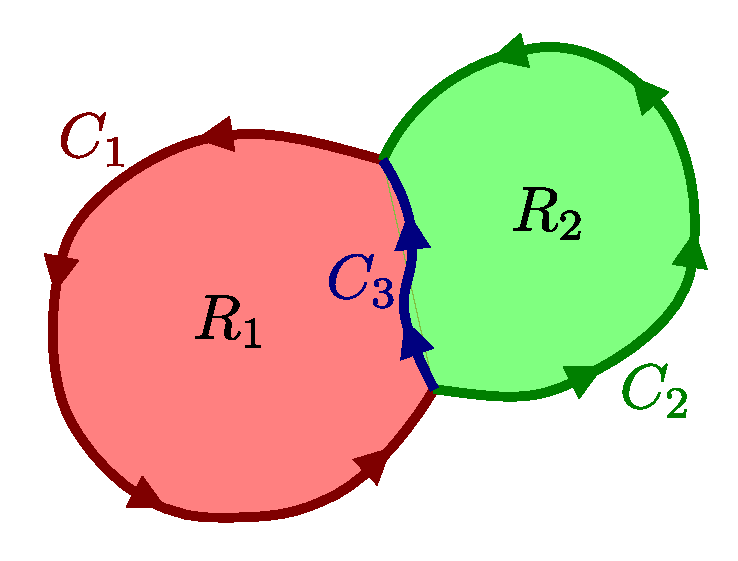
\includegraphics[width = 0.5\textwidth]{loop_sum}
}
\end{tabular}

The counterclockwise boundaries of \(R_1\) and \(R_2\) are respectively:
\[\text{boundary}(R_1) = C_1 + C_3 \quad\quad\text{and}\quad\quad \text{boundary}(R_2) = C_2 - C_3\]
(note the reversal of the orientation of \(C_3\) in the boundary of \(R_2\))

The counterclockwise boundary of the union of \(R_1\) and \(R_2\) is:
\[\text{boundary}(R_1 \cup R_2) = C_1 + C_2\]

The vector loop integrals of \(\mathbf{F}(\mathbf{q})\) around the counterclockwise boundaries of \(R_1\), \(R_2\), and \(R_1 \cup R_2\) are respectively:
\[\oint_{\text{boundary}(R_1)} \mathbf{F}(\mathbf{q}) \bullet d\mathbf{q} = \oint_{C_1 + C_3} \mathbf{F}(\mathbf{q}) \bullet d\mathbf{q} = \int_{C_1} \mathbf{F}(\mathbf{q}) \bullet d\mathbf{q} + \int_{C_3} \mathbf{F}(\mathbf{q}) \bullet d\mathbf{q}\]
\[\oint_{\text{boundary}(R_2)} \mathbf{F}(\mathbf{q}) \bullet d\mathbf{q} = \oint_{C_2 - C_3} \mathbf{F}(\mathbf{q}) \bullet d\mathbf{q} = \int_{C_2} \mathbf{F}(\mathbf{q}) \bullet d\mathbf{q} - \int_{C_3} \mathbf{F}(\mathbf{q}) \bullet d\mathbf{q}\]
\[\oint_{\text{boundary}(R_1 \cup R_2)} \mathbf{F}(\mathbf{q}) \bullet d\mathbf{q} = \oint_{C_1 + C_2} \mathbf{F}(\mathbf{q}) \bullet d\mathbf{q} = \int_{C_1} \mathbf{F}(\mathbf{q}) \bullet d\mathbf{q} + \int_{C_2} \mathbf{F}(\mathbf{q}) \bullet d\mathbf{q}\]
Therefore:
\[\oint_{\text{boundary}(R_1 \cup R_2)} \mathbf{F}(\mathbf{q}) \bullet d\mathbf{q} = \oint_{\text{boundary}(R_1)} \mathbf{F}(\mathbf{q}) \bullet d\mathbf{q} + \oint_{\text{boundary}(R_2)} \mathbf{F}(\mathbf{q}) \bullet d\mathbf{q}\]

\begin{tabular}{cc}
\parbox{0.5\textwidth}{
The circulation around the counterclockwise boundary of the union of two 2D regions is the sum of the circulations around the counterclockwise boundaries of the two regions individually. Generalizing upon this observation, an arbitrary 2D region \(R\) can be decomposed into a number of tiny regions. The circulation around the counterclockwise boundary \(C\) of \(R\) is the sum of the circulations around the counterclockwise boundaries of these tiny regions. 
} & \parbox{0.5\textwidth}{
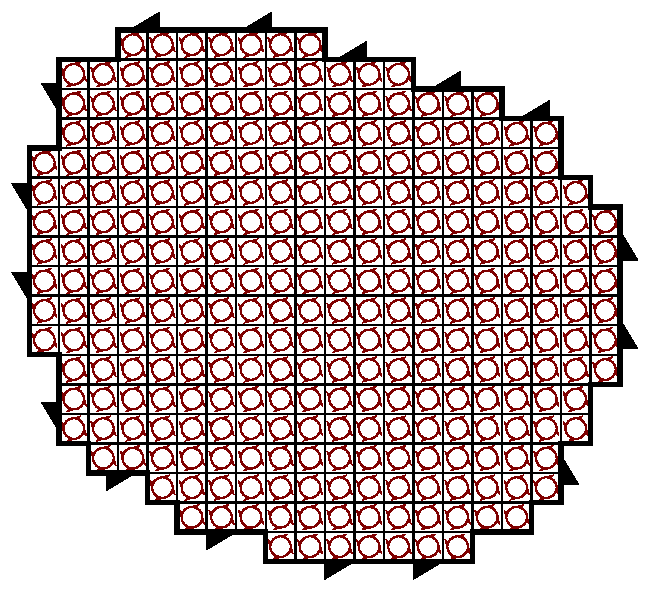
\includegraphics[width = 0.5\textwidth]{2D_loop_decomposition_x}
}
\end{tabular}

\begin{tabular}{cc}
\parbox{0.5\textwidth}{
Each tiny region is an infinitesimal rectangle. Let \(N\) be a large number that denotes the number of rectangles. For each \(i = 1, 2, ..., N\), let rectangle \(i\) be centered on the point \((x_i^*, y_i^*)\), have a width of \(\Delta x_i\) and a height of \(\Delta y_i\).  The rectangle covers the \(x\) coordinate range \([x_{L,i}, x_{U,i}]\) and the \(y\) coordinate range \([y_{L,i}, y_{U,i}]\). The rectangle has \(4\) sides: bottom, right, top, and left, and its boundary \(C_i = \text{bottom} + \text{right} + \text{top} + \text{left}\) has a counterclockwise orientation. The vector line integral of \(\mathbf{F}(x,y) = \begin{bmatrix} F_x(x,y) \\ F_y(x,y) \end{bmatrix}\) along each side will each be approximated by a single dot product. 
} & \parbox{0.5\textwidth}{
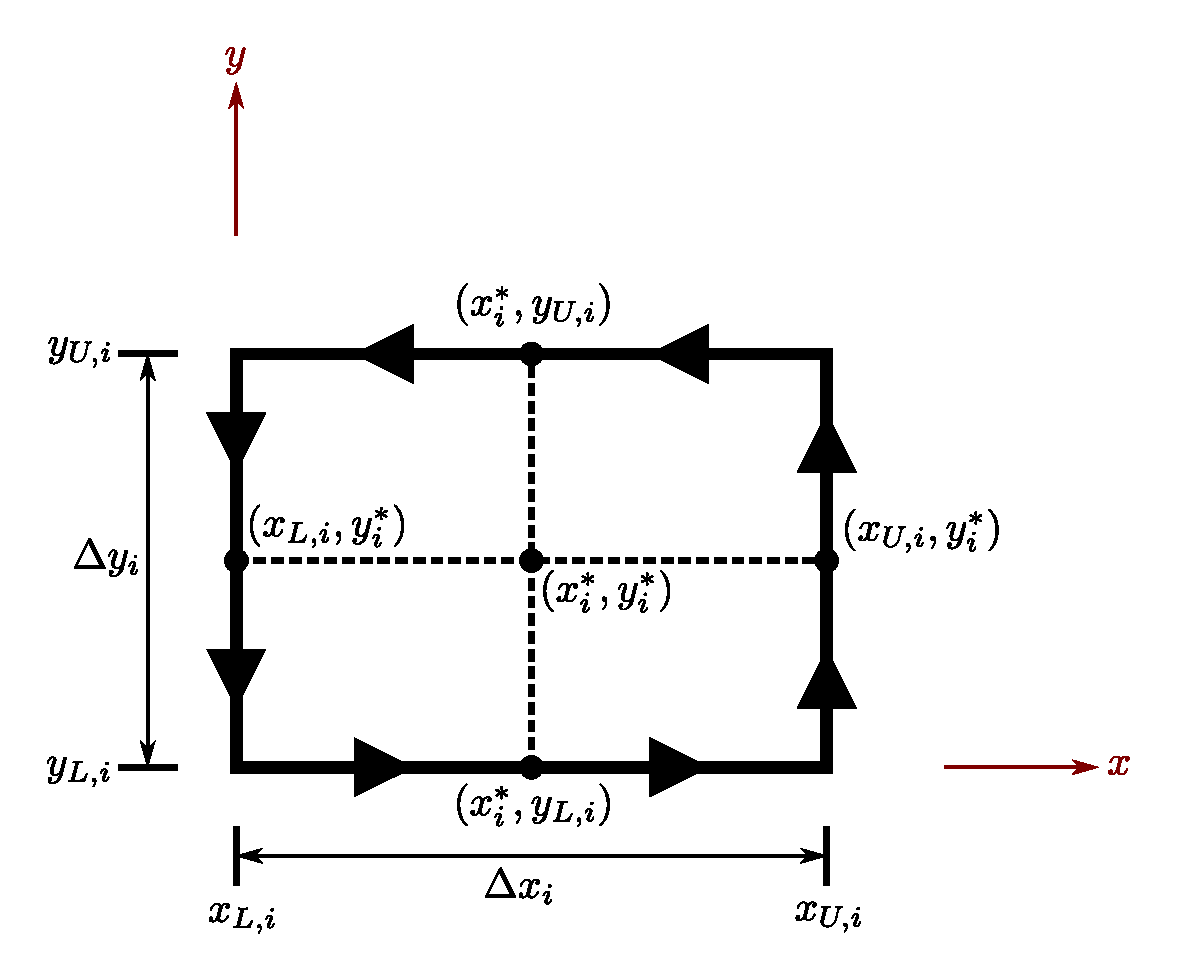
\includegraphics[width = 0.5\textwidth]{infinitesimal_rectangle}
}
\end{tabular}

The bottom has the ``average point" \((x_i^*, y_{L,i})\) and a total displacement of \(\begin{bmatrix} \Delta x_i \\ 0 \end{bmatrix}\) so: 
\[\int_{\text{bottom}} \mathbf{F}(x,y) \bullet d\mathbf{q} = \int_{\text{bottom}} \begin{bmatrix} F_x(x,y) \\ F_y(x,y) \end{bmatrix} \bullet \begin{bmatrix} dx \\ dy \end{bmatrix} \approx \begin{bmatrix} F_x(x_i^*, y_{L,i}) \\ F_y(x_i^*, y_{L,i}) \end{bmatrix} \bullet \begin{bmatrix} \Delta x_i \\ 0 \end{bmatrix} = F_x(x_i^*, y_{L,i}) \Delta x_i\]

The right has the ``average point" \((x_{U,i}, y_i^*)\) and a total displacement of \(\begin{bmatrix} 0 \\ \Delta y_i \end{bmatrix}\) so: 
\[\int_{\text{right}} \mathbf{F}(x,y) \bullet d\mathbf{q} = \int_{\text{right}} \begin{bmatrix} F_x(x,y) \\ F_y(x,y) \end{bmatrix} \bullet \begin{bmatrix} dx \\ dy \end{bmatrix} \approx \begin{bmatrix} F_x(x_{U,i}, y_i^*) \\ F_y(x_{U,i}, y_i^*) \end{bmatrix} \bullet \begin{bmatrix} 0 \\ \Delta y_i \end{bmatrix} = F_y(x_{U,i}, y_i^*) \Delta y_i\]

The top has the ``average point" \((x_i^*, y_{U,i})\) and a total displacement of \(\begin{bmatrix} -\Delta x_i \\ 0 \end{bmatrix}\) so: 
\[\int_{\text{top}} \mathbf{F}(x,y) \bullet d\mathbf{q} = \int_{\text{top}} \begin{bmatrix} F_x(x,y) \\ F_y(x,y) \end{bmatrix} \bullet \begin{bmatrix} dx \\ dy \end{bmatrix} \approx \begin{bmatrix} F_x(x_i^*, y_{U,i}) \\ F_y(x_i^*, y_{U,i}) \end{bmatrix} \bullet \begin{bmatrix} -\Delta x_i \\ 0 \end{bmatrix} = -F_x(x_i^*, y_{U,i}) \Delta x_i\]

The left has the ``average point" \((x_{L,i}, y_i^*)\) and a total displacement of \(\begin{bmatrix} 0 \\ -\Delta y_i \end{bmatrix}\) so: 
\[\int_{\text{left}} \mathbf{F}(x,y) \bullet d\mathbf{q} = \int_{\text{left}} \begin{bmatrix} F_x(x,y) \\ F_y(x,y) \end{bmatrix} \bullet \begin{bmatrix} dx \\ dy \end{bmatrix} \approx \begin{bmatrix} F_x(x_{L,i}, y_i^*) \\ F_y(x_{L,i}, y_i^*) \end{bmatrix} \bullet \begin{bmatrix} 0 \\ -\Delta y_i \end{bmatrix} = -F_y(x_{L,i}, y_i^*) \Delta y_i\]

In total, 
\begin{align*}
\oint_{C_i} \mathbf{F}(x,y) \bullet d\mathbf{q} = & 
\oint_{\text{bottom} + \text{right} + \text{top} + \text{left}} \mathbf{F}(x,y) \bullet d\mathbf{q} \\ 
= & \oint_{\text{bottom}} \mathbf{F}(x,y) \bullet d\mathbf{q} + \oint_{\text{right}} \mathbf{F}(x,y) \bullet d\mathbf{q} + \oint_{\text{top}} \mathbf{F}(x,y) \bullet d\mathbf{q} + \oint_{\text{left}} \mathbf{F}(x,y) \bullet d\mathbf{q} \\ 
\approx & F_x(x_i^*, y_{L,i}) \Delta x_i + F_y(x_{U,i}, y_i^*) \Delta y_i - F_x(x_i^*, y_{U,i}) \Delta x_i - F_y(x_{L,i}, y_i^*) \Delta y_i \\   
= & \Delta x_i \Delta y_i \left(\frac{F_y(x_{U,i}, y_i^*) - F_y(x_{L,i}, y_i^*)}{\Delta x_i} - \frac{F_x(x_i^*, y_{U,i}) - F_x(x_i^*, y_{L,i})}{\Delta y_i}\right) 
\end{align*}
The quotients \(\frac{F_y(x_{U,i}, y_i^*) - F_y(x_{L,i}, y_i^*)}{\Delta x_i}\) and \(\frac{F_x(x_i^*, y_{U,i}) - F_x(x_i^*, y_{L,i})}{\Delta y_i}\) respectively approximate the partial derivatives \(\left.\frac{\partial F_y}{\partial x}\right|_{(x_i^*, y_i^*)}\) and \(\left.\frac{\partial F_x}{\partial y}\right|_{(x_i^*, y_i^*)}\). Therefore:
\[\oint_{C_i} \mathbf{F}(x,y) \bullet d\mathbf{q} \approx \Delta x_i \Delta y_i \left(\left.\frac{\partial F_y}{\partial x}\right|_{(x_i^*, y_i^*)} - \left.\frac{\partial F_x}{\partial y}\right|_{(x_i^*, y_i^*)}\right)\]

The total circulation of the vector field \(\mathbf{F}(x, y) = \begin{bmatrix} F_x(x,y) \\ F_y(x,y) \end{bmatrix}\) around the counterclockwise boundary \(C\) of 2D region \(R\) is the sum of the circulation around the counterclockwise boundaries of each infinitesimal rectangle: 

\begin{align*}
\oint_C \mathbf{F}(x,y) \bullet d\mathbf{q} = & \lim_{N \rightarrow +\infty} \sum_{i = 1}^N \oint_{C_i} \mathbf{F}(x,y) \bullet d\mathbf{q} \\ 
= & \lim_{N \rightarrow +\infty} \sum_{i = 1}^N \Delta x_i \Delta y_i \left(\left.\frac{\partial F_y}{\partial x}\right|_{(x_i^*, y_i^*)} - \left.\frac{\partial F_x}{\partial y}\right|_{(x_i^*, y_i^*)}\right) \\ 
= & \iint_R \left(\frac{\partial F_y}{\partial x} - \frac{\partial F_x}{\partial y}\right)dA
\end{align*}

The equation 
\[\oint_C \begin{bmatrix} F_x(x,y) \\ F_y(x,y) \end{bmatrix} \bullet d\mathbf{q} = \iint_R \left(\frac{\partial F_y}{\partial x} - \frac{\partial F_x}{\partial y}\right)dA\]
is referred to as {\bf Green's theorem}. Green's theorem allows the conversion of an otherwise complicated vector loop integral to a simpler double integral.

The quantity \(\frac{\partial F_y}{\partial x} - \frac{\partial F_x}{\partial y}\) can be thought of as the ``circulation density" of the vector field \(\mathbf{F}(x,y) = \begin{bmatrix} F_x(x,y) \\ F_y(x,y) \end{bmatrix}\). The total circulation around the counterclockwise boundary of a region \(R\) is the double integral of the circulation density inside of \(R\). The circulation density is also referred to as the {\bf curl} of the vector field \(\mathbf{F}(x,y) = \begin{bmatrix} F_x(x,y) \\ F_y(x,y) \end{bmatrix}\). 

\vspace{5mm}

\textbf{Examples:}

\begin{itemize}
%%%%%%%%%%%%%%%%%%%%%%%%%%%%%%%%%%%
\item Find the vector loop integral:
\[\oint_C \begin{bmatrix} x^3 - 2y \\ 5x - y^2 \end{bmatrix} \bullet d\mathbf{q}\]
where loop \(C\) is the counterclockwise perimeter of the rectangle with the vertices \((0, 0)\), \((3, 0)\), \((3, 2)\), and \((0, 2)\).

The ``circulation density" of the vector field \(\begin{bmatrix} F_x(x,y) \\ F_y(x,y) \end{bmatrix} = \begin{bmatrix} x^3 - 2y \\ 5x - y^2 \end{bmatrix}\) is: 
\begin{align*}
\frac{\partial F_y}{\partial x} - \frac{\partial F_x}{\partial y} = & \frac{\partial}{\partial x}(5x - y^2) - \frac{\partial}{\partial y}(x^3 - 2y) = 5 - (-2) = 7 
\end{align*}

The interior of the rectangle is the region:
\[R = \{(x,y) | 0 \leq x \leq 3 \;\&\; 0 \leq y \leq 2\}\] 

The total circulation is the double integral of the circulation density over \(R\):
\begin{align*}
& \oint_C \begin{bmatrix} x^3 - 2y \\ 5x - y^2 \end{bmatrix} \bullet d\mathbf{q} 
= \oint_C \begin{bmatrix} F_x(x,y) \\ F_y(x,y) \end{bmatrix} \bullet d\mathbf{q} 
= \iint_R \left(\frac{\partial F_y}{\partial x} - \frac{\partial F_x}{\partial y}\right)dA \\ 
& = \iint_R 7 dA 
= \int_{x = 0}^3 \left(\int_{y = 0}^2 7dy\right)dx 
= \int_{x = 0}^3 7y\Big|_{y = 0}^2 dx 
= \int_{x = 0}^3 14 dx 
= 14x\Big|_{x = 0}^3 
= 42
\end{align*}

%%%%%%%%%%%%%%%%%%%%%%%%%%%%%%%%%%%
\item Find the vector loop integral:
\[\oint_C \begin{bmatrix} 2xy + \cos(x^2) \\ xy - \ln(y + 1) \end{bmatrix} \bullet d\mathbf{q}\]
where loop \(C\) is the counterclockwise perimeter of the triangle with the vertices \((0, 0)\), \((3, 0)\), and \((0, 2)\).

The ``circulation density" of the vector field \(\begin{bmatrix} F_x(x,y) \\ F_y(x,y) \end{bmatrix} = \begin{bmatrix} 2xy + \cos(x^2) \\ xy - \ln(y + 1) \end{bmatrix}\) is: 
\begin{align*}
\frac{\partial F_y}{\partial x} - \frac{\partial F_x}{\partial y} = & \frac{\partial}{\partial x}(xy - \ln(y + 1)) - \frac{\partial}{\partial y}(2xy + \cos(x^2)) = y - 2x  
\end{align*}

The interior of the triangle is the region:
\[R = \left\{(x,y) \middle| 0 \leq x \leq 3 \;\&\; 0 \leq y \leq 2 - \frac{2}{3}x\right\}\] 

The total circulation is the double integral of the circulation density over \(R\):
\begin{align*}
& \oint_C \begin{bmatrix} 2xy + \cos(x^2) \\ xy - \ln(y + 1) \end{bmatrix} \bullet d\mathbf{q} 
= \oint_C \begin{bmatrix} F_x(x,y) \\ F_y(x,y) \end{bmatrix} \bullet d\mathbf{q} 
= \iint_R \left(\frac{\partial F_y}{\partial x} - \frac{\partial F_x}{\partial y}\right)dA \\ 
& = \iint_R (y - 2x) dA 
= \int_{x = 0}^3 \left(\int_{y = 0}^{2 - \frac{2}{3}x} (y - 2x)dy\right)dx 
= \int_{x = 0}^3 (\frac{1}{2}y^2 - 2xy)\Big|_{y = 0}^{2 - \frac{2}{3}x} dx \\ 
& = \int_{x = 0}^3 (\frac{1}{2}(4 - \frac{8}{3}x + \frac{4}{9}x^2) - 2x(2 - \frac{2}{3}x))dx 
= \int_{x = 0}^3 ((2 - \frac{4}{3}x + \frac{2}{9}x^2) + (-4x + \frac{4}{3}x^2))dx \\
& = \int_{x = 0}^3 (2 - \frac{16}{3}x + \frac{14}{9}x^2)dx 
= (2x - \frac{8}{3}x^2 + \frac{14}{27}x^3)\Big|_{x = 0}^3 
= (6 - 24 + 14) - 0 
= -4
\end{align*}

%%%%%%%%%%%%%%%%%%%%%%%%%%%%%%%%%%%
\item Find the vector loop integral:
\[\oint_C \begin{bmatrix} 2x \\ \ln(x + 1) - y \end{bmatrix} \bullet d\mathbf{q}\]
where loop \(C\) is the counterclockwise perimeter of the parallelogram with the vertices \((0, -3)\), \((5, 0)\), \((5, 3)\), and \((0, 0)\).

The ``circulation density" of the vector field \(\begin{bmatrix} F_x(x,y) \\ F_y(x,y) \end{bmatrix} = \begin{bmatrix} 2x \\ \ln(x + 1) - y \end{bmatrix}\) is: 
\begin{align*}
\frac{\partial F_y}{\partial x} - \frac{\partial F_x}{\partial y} = & \frac{\partial}{\partial x}(\ln(x + 1) - y) - \frac{\partial}{\partial y}(2x) = \frac{1}{x + 1} - 0 = \frac{1}{x + 1} 
\end{align*}

The interior of the parallelogram is the region:
\[R = \left\{(x,y) \middle| 0 \leq x \leq 5 \;\&\; -3 + \frac{3}{5}x \leq y \leq \frac{3}{5}x\right\}\] 

The total circulation is the double integral of the circulation density over \(R\):
\begin{align*}
& \oint_C \begin{bmatrix} 2x \\ \ln(x + 1) - y \end{bmatrix} \bullet d\mathbf{q} 
= \oint_C \begin{bmatrix} F_x(x,y) \\ F_y(x,y) \end{bmatrix} \bullet d\mathbf{q} 
= \iint_R \left(\frac{\partial F_y}{\partial x} - \frac{\partial F_x}{\partial y}\right)dA \\ 
& = \iint_R \frac{1}{x + 1} dA 
= \int_{x = 0}^5 \left(\int_{y = -3 + \frac{3}{5}x}^{\frac{3}{5}x} \frac{1}{x + 1}dy\right)dx 
= \int_{x = 0}^5 \frac{y}{x+1}\Big|_{y = -3 + \frac{3}{5}x}^{\frac{3}{5}x} dx \\ 
& = \int_{x = 0}^5 \left(\frac{3x}{5x + 5} - \frac{3x - 15}{5x + 5}\right)dx 
= \int_{x = 0}^5 \frac{15}{5x + 5} dx 
= \int_{x = 0}^5 \frac{3}{x + 1} dx 
= 3\ln(x + 1)\Big|_{x = 0}^5 \\
& = 3\ln(6) - 3\ln(1) 
= 3\ln(6)
\end{align*}

%%%%%%%%%%%%%%%%%%%%%%%%%%%%%%%%%%%
\item Find the vector loop integral:
\[\oint_C \begin{bmatrix} -x^2 + y^2 \\ 8xy + 3y^2 \end{bmatrix} \bullet d\mathbf{q}\]
where loop \(C\) is the counterclockwise perimeter of the triangle with the vertices \((-1, 0)\), \((3, 0)\), and \((0, 2)\).

The ``circulation density" of the vector field \(\begin{bmatrix} F_x(x,y) \\ F_y(x,y) \end{bmatrix} = \begin{bmatrix} -x^2 + y^2 \\ 8xy + 3y^2 \end{bmatrix}\) is: 
\begin{align*}
\frac{\partial F_y}{\partial x} - \frac{\partial F_x}{\partial y} = & \frac{\partial}{\partial x}(8xy + 3y^2) - \frac{\partial}{\partial y}(-x^2 + y^2) = 8y - 2y = 6y 
\end{align*}

The interior of the parallelogram is the region:
\[R = \left\{(x,y) \middle| 0 \leq y \leq 2 \;\&\; -1 + \frac{1}{2}y \leq x \leq 3 - \frac{3}{2}y\right\}\] 

The total circulation is the double integral of the circulation density over \(R\):
\begin{align*}
& \oint_C \begin{bmatrix} -x^2 + y^2 \\ 8xy + 3y^2 \end{bmatrix} \bullet d\mathbf{q} 
= \oint_C \begin{bmatrix} F_x(x,y) \\ F_y(x,y) \end{bmatrix} \bullet d\mathbf{q} 
= \iint_R \left(\frac{\partial F_y}{\partial x} - \frac{\partial F_x}{\partial y}\right)dA \\ 
& = \iint_R 6y dA 
= \int_{y = 0}^2 \left(\int_{x = -1 + \frac{1}{2}y}^{3 - \frac{3}{2}y} 6y dx\right)dy 
= \int_{y = 0}^2 6xy\Big|_{x = -1 + \frac{1}{2}y}^{3 - \frac{3}{2}y} dy \\ 
& = \int_{y = 0}^2 ((18y - 9y^2) - (-6y + 3y^2))dy 
= \int_{y = 0}^2 (24y - 12y^2) dy 
= (12y^2 - 4y^3)\Big|_{y = 0}^2 
= (48 - 32) - 0 \\
& = 16
\end{align*}
\end{itemize}



\section*{The divergence theorem}

Often vector fields denote ``flow density". Flow density describes the movement of liquids. The direction of the vector field \(\mathbf{F}(\mathbf{q})\) at point \(\mathbf{q}\) is the direction that the fluid is flowing at point \(\mathbf{q}\), while the magnitude \(\|\mathbf{F}(\mathbf{q})\|\) is a measure of the rate of flow through a unit cross section that is oriented perpendicular (head on) to the direction of flow. 

\begin{tabular}{cc}
\parbox{0.5\textwidth}{
Given an oriented curve \(C\) in 2D space, a sought after quantity is the total flow across curve \(C\). The flow that will be computed will cross the curve from a ``left to right" fashion. Partition the curve into a large number \(N\) of infinitesimal sections. Section \(i\) has the representative point \(\mathbf{q}_i^*\) and spans the displacement \(\Delta\mathbf{q}_i = \begin{bmatrix} \Delta x_i \\ \Delta y_i \end{bmatrix}\). The component of \(\Delta\mathbf{q}_i\) that is perpendicular to the local flow density \(\mathbf{F}(\mathbf{q}_i^*)\) has a length of \(\|\Delta\mathbf{q}_i\|\cos\theta\) where \(\theta\) is the angle between \(\Delta\mathbf{q}_i\) and a direction that is orthogonal to the local flow density. Why is a direction that is orthogonal to the flow density important? \(\|\mathbf{F}(\mathbf{q}_i^*)\|\) is a measure of the rate of flow through a unit cross section that is oriented perpendicular (head on) to the direction of flow. Details are depicted on the right. 

\(\theta\) is not a measure of the angle between \(\Delta\mathbf{q}_i\) and \(\mathbf{F}(\mathbf{q}_i^*)\). \(\theta\) is however, a measure of the angle between \(\Delta\mathbf{S}_i\) and \(\mathbf{F}(\mathbf{q}_i^*)\) where \(\Delta\mathbf{S}_i\) is a clockwise \(90^\circ\) rotation of \(\Delta\mathbf{q}_i\). \(\Delta\mathbf{q}_i\) and \(\Delta\mathbf{S}_i\) have equal lengths.       
} & \parbox{0.5\textwidth}{
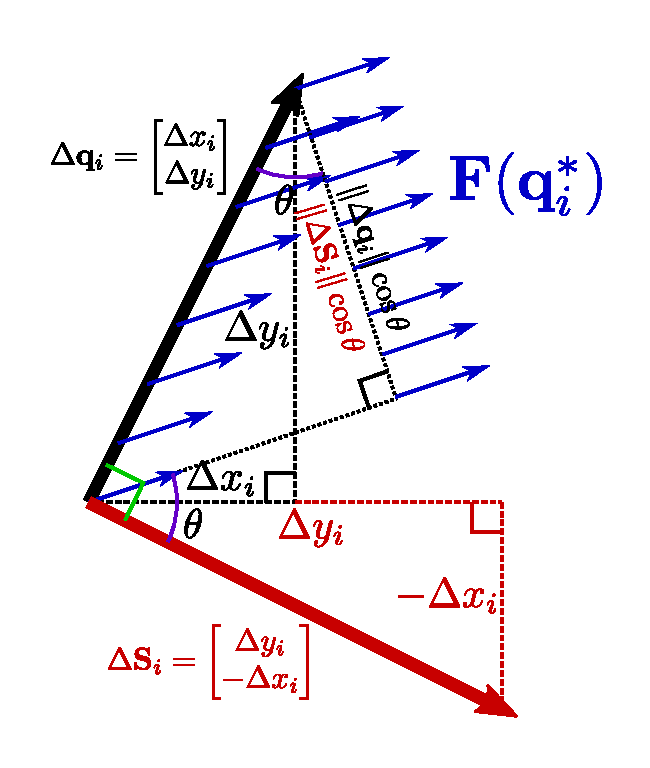
\includegraphics[width = 0.5\textwidth]{flux_through_dq}
}
\end{tabular}

Moreover, \(\Delta\mathbf{S}_i = \begin{bmatrix} \Delta y_i \\ -\Delta x_i \end{bmatrix}\). 

Putting everything together, the flow across \(\Delta\mathbf{q}_i\) is 
\[(\|\Delta\mathbf{q}_i\|\cos\theta)\|\mathbf{F}(\mathbf{q}_i^*)\| = \|\mathbf{F}(\mathbf{q}_i^*)\|\|\Delta\mathbf{S}_i\|\cos\theta = \mathbf{F}(\mathbf{q}_i^*) \bullet \Delta\mathbf{S}_i = \mathbf{F}(\mathbf{q}_i^*) \bullet \begin{bmatrix} \Delta y_i \\ -\Delta x_i \end{bmatrix}\]

The left to right flow across curve \(C\) is
\begin{align*}
& \lim_{N \rightarrow +\infty} \sum_{i = 1}^N \mathbf{F}(\mathbf{q}_i^*) \bullet \begin{bmatrix} \Delta y_i \\ -\Delta x_i \end{bmatrix}
= \int_C \mathbf{F}(\mathbf{q}) \bullet \begin{bmatrix} dy \\ -dx \end{bmatrix}
\end{align*}

The ``flux integral" \(\int_C \mathbf{F}(\mathbf{q}) \bullet \begin{bmatrix} dy \\ -dx \end{bmatrix}\) can be rewritten as a ``standard" vector line integral via: 
\begin{align*}
& \int_C \begin{bmatrix} F_x(x,y) \\ F_y(x,y) \end{bmatrix} \bullet \begin{bmatrix} dy \\ -dx \end{bmatrix} 
= \int_C (F_x(x,y)dy - F_y(x,y)dx) 
= \int_C ((-F_y(x,y))dx + F_x(x,y)dy) \\
& = \int_C \begin{bmatrix} -F_y(x,y) \\ F_x(x,y) \end{bmatrix} \bullet \begin{bmatrix} dx \\ dy \end{bmatrix}
= \int_C \begin{bmatrix} -F_y(x,y) \\ F_x(x,y) \end{bmatrix} \bullet d\mathbf{q} 
\end{align*}
Therefore:
\[\int_C \begin{bmatrix} F_x(x,y) \\ F_y(x,y) \end{bmatrix} \bullet \begin{bmatrix} dy \\ -dx \end{bmatrix} = \int_C \begin{bmatrix} -F_y(x,y) \\ F_x(x,y) \end{bmatrix} \bullet d\mathbf{q}\]

If \(C\) is the counterclockwise orient boundary of a 2D region \(R\), then the total flow that is {\bf leaving} \(R\) is:
\begin{align*}
& \oint_C \begin{bmatrix} F_x(x,y) \\ F_y(x,y) \end{bmatrix} \bullet \begin{bmatrix} dy \\ -dx \end{bmatrix} 
= \oint_C \begin{bmatrix} -F_y(x,y) \\ F_x(x,y) \end{bmatrix} \bullet d\mathbf{q} \\ 
& = \iint_R \left(\frac{\partial}{\partial x}(F_x(x,y)) - \frac{\partial}{\partial y}(-F_y(x,y))\right)dA \quad\quad\text{(using Green's theorem)} \\
& = \iint_R \left(\frac{\partial F_x}{\partial x} + \frac{\partial F_y}{\partial y}\right)dA
\end{align*}

The equation
\[\oint_C \begin{bmatrix} F_x(x,y) \\ F_y(x,y) \end{bmatrix} \bullet \begin{bmatrix} dy \\ -dx \end{bmatrix} = \iint_R \left(\frac{\partial F_x}{\partial x} + \frac{\partial F_y}{\partial y}\right)dA\]
is referred to as the {\bf Divergence theorem}. 

The quantity \(\frac{\partial F_x}{\partial x} + \frac{\partial F_y}{\partial y}\) is the {\bf divergence} of the vector field \(\mathbf{F}(x,y) = \begin{bmatrix} F_x(x,y) \\ F_y(x,y) \end{bmatrix}\) and is denoted by the notation \(\nabla \bullet \mathbf{F}\):
\[\nabla \bullet \mathbf{F} = \frac{\partial F_x}{\partial x} + \frac{\partial F_y}{\partial y}\]
The divergence is the ``flow generation density". The divergence theorem states that the total flow leaving a region \(R\) across its boundary \(C\) is the total rate of flow generation inside of \(R\).




\end{document}















